\documentclass[12pt,a4paper]{amsart}
\usepackage[utf8]{inputenc}
\usepackage[T1]{fontenc}
\usepackage{amsmath,amssymb,amsthm}
\usepackage{booktabs}
\usepackage{graphicx}
\usepackage{array}
\usepackage{enumitem}
\usepackage[margin=1in]{geometry}
\usepackage{xcolor}
\usepackage{float}
\usepackage{multirow}
\usepackage{hyperref}
\hypersetup{colorlinks=true,linkcolor=blue!60!black,citecolor=blue!60!black,urlcolor=blue!60!black,
  pdftitle={Prime polynomials in Legendre intervals over F(2k)[t], III: the hexad of a quartic linearised polynomial, the symplectic group Sp4(F2), and the Witt sums behind the constant X},
  pdfauthor={Ruqing Chen}}

\newtheorem{theorem}{Theorem}[section]
\newtheorem{proposition}[theorem]{Proposition}
\newtheorem{lemma}[theorem]{Lemma}
\newtheorem{corollary}[theorem]{Corollary}
\newtheorem{conjecture}[theorem]{Conjecture}
\theoremstyle{definition}
\newtheorem{definition}[theorem]{Definition}
\newtheorem{remark}[theorem]{Remark}
\newtheorem{example}[theorem]{Example}

\newcommand{\F}{\mathbb{F}}
\newcommand{\Z}{\mathbb{Z}}
\newcommand{\Q}{\mathbb{Q}}
\newcommand{\A}{\mathbb{A}}
\newcommand{\G}{\mathcal{G}}
\newcommand{\Tr}{\operatorname{Tr}}
\newcommand{\Var}{\operatorname{Var}}
\newcommand{\Arf}{\operatorname{Arf}}
\newcommand{\im}{\operatorname{im}}
\newcommand{\Sp}{\operatorname{Sp}}
\newcommand{\GL}{\operatorname{GL}}
\newcommand{\Sw}{\operatorname{Sw}}
\newcommand{\Br}{\operatorname{Br}}
\newcommand{\eps}{\varepsilon}
\newcommand{\Kk}{\mathcal{K}}
\newcommand{\Rr}{\mathcal{R}}
\newcommand{\qq}{\mathfrak{q}}
\newcommand{\Spp}{S''}
\emergencystretch=1.5em

\title[Legendre intervals in even characteristic, III]{Prime polynomials in Legendre intervals over \texorpdfstring{$\F_{2^k}[t]$}{F(2k)[t]}, III:\texorpdfstring{\\}{ }the hexad of a quartic linearised polynomial, the symplectic group \texorpdfstring{$\Sp_4(\F_2)$}{Sp4(F2)}, and the Witt sums behind the constant \texorpdfstring{$X$}{X}}

\author{Ruqing Chen}
\address{GUT Geoservice Inc., Montreal, Canada}
\email{ruqing@hotmail.com}
\thanks{Preprint. Code and data: \url{https://github.com/Ruqing1963/legendre-intervals-part2} (directory \texttt{paper3/} and the scripts named in Section~\ref{sec:numerics}). Part~II: DOI 10.5281/zenodo.23252762.}
\date{\today}

\begin{document}

\begin{abstract}
Let $q=2^k$ with $k$ odd. Part~II of this series reduced the second of the three constants governing the variance of prime polynomials in Legendre intervals at degree $d=6$, $X=\sum_{\alpha\in U}\chi(e_2(\alpha))$ with $U=\{\alpha\in\F_{q^{12}}:\Tr\alpha=\Tr\alpha^3=\Tr\alpha^5=0\}$, to sums $W'(\lambda_3,\lambda_5)$ of characters of order $4$ of the Hayes group, whose fine structure is governed by the kernel of the linearised polynomial $L'_\lambda(x)=\lambda_5^4x^{16}+\lambda_3^4x^8+x^4+\lambda_3^2x^2+\lambda_5x$. Numerically, the Frobenius acted on this four-dimensional $\F_2$-space through $\Sp_4(\F_2)\cong S_6$ with exact polynomial class frequencies, and $W'$ was a function of the class. This paper explains the phenomenon and proves a substantial part of it. The kernel of $L'_\lambda$ is the set of pairwise sums of the six roots of the sextic
\[
B_\lambda(u)=\lambda_5^2u^6+\lambda_3^2u^2+\lambda_5u+1=u\,A_\lambda(u)+1,
\]
where $A_\lambda$ is the Bluher quintic whose roots span the kernel of the quadratic-character analogue $L_\lambda=L'_\lambda-x^4$; the proof is the identity $L'_\lambda=x^4B_\lambda^2+B_\lambda+1$ together with a division of $B_\lambda$ by a quadratic factor. Consequently the Frobenius permutes the six roots, the $S_6$-class is the factorisation type of $B_\lambda$ over $\F_q$, the symplectic form is the duad--syntheme pairing of the generalised quadrangle $W(2)$, the roots are six of the sixteen elements of the coset $T_\lambda'^{-1}(1)$ of the polar operator, and the one-parameter deformation $L_\lambda+\eps x^4$ corresponds to $uA_\lambda(u)+\sqrt\eps$, interpolating between the quadratic sums of $A_6$ and the order-$4$ sums of $X$. We prove the first moment identities of the family (the numbers of roots in $\F_q$, of ordered pairs of roots in $\F_q$, and of roots in $\F_{q^2}\setminus\F_q$ total $(q-1)^2$, $(q-2)^2$ and $q(q-2)$) and verify the eleven class counts up to $q=512$. The order-$4$ sums are then treated as Frobenius traces of rank-four Witt--Artin--Schreier sheaves. Using the hexad, a multiplicity formula for Witt traces along towers, and the moduli of Gauss sums of $\Z/4$-valued quadratic forms, we prove: every individual sum $\Spp(\lambda)$ is a rational integer; the normalised Frobenius eigenvalues are roots of unity; in the class of $5$-cycles the $L$-polynomial is $(1-\eta^5q^{5/2}T^5)/(1-\eta q^{1/2}T)$ with $\eta$ a \emph{primitive} $8$th root of unity, so that $\Spp(\lambda)=-q^6$ for every $\lambda$ and $W'=-q^7$, the term carrying the leading constant of $X$; in the six classes whose kernel lies in $\F_{q^4}$ the sum over $\F_{q^{12}}$ equals $q^4$ times the sum over $\F_{q^4}$; in the remaining classes every $\Spp(\lambda)$ equals $\pm4q^6$. The closed form $X=q^6+q^5$ is thereby reduced to the class counts and to the Brown invariants of explicit $\Z/4$-valued forms over $\F_{q^4}$ and $\F_{q^6}$, all stated precisely and verified for $q\le128$.
\end{abstract}

\maketitle
\tableofcontents

\section{Introduction}

\subsection{Background}
Let $q=2^k$, $d\ge2$, $n=2d$, and let $\G=\G_{d-1}=\{1+c_1u+\dots+c_{d-1}u^{d-1}\}$ be the Hayes group of truncated power series over $\F_q$, which classifies monic polynomials of degree $n$ by their top $d-1$ coefficients. The Legendre interval of a monic $f$ of degree $d$ is $\mathcal I_f=\{f^2+s:\deg s\le d\}$, the fibre over the class of $f^2$; in characteristic $2$ these classes form the subgroup $\G^2$ of squares, of index $q^{\lfloor d/2\rfloor}$, and the variance of the prime-power count $\Psi(f)=\sum_{P\in\mathcal I_f}\Lambda(P)$ over Legendre intervals is amplified by a factor $\asymp q^2$ at $d=4$ and $d=6$ relative to the Keating--Rudnick value for the full group \cite{Chen,ChenII}. At $d=6$ Part~II \cite{ChenII} proved that $\Psi$ takes exactly three values on the $q^2$ Legendre classes and that the variance is an explicit function of three constants
\begin{gather*}
A_6=|U|,\qquad X=\sum_{\alpha\in U}\chi(e_2(\alpha)),\qquad Y=\sum_{\alpha\in U}\chi(e_4(\alpha)),\\
U=\{\alpha\in\F_{q^{12}}:\Tr\alpha=\Tr\alpha^3=\Tr\alpha^5=0\},
\end{gather*}
where $\chi=(-1)^{\Tr_{q/2}}$ and $e_j(\alpha)$ is the $j$-th elementary symmetric function of the twelve conjugates of $\alpha$ over $\F_q$; explicitly (Part~II, \S8)
\[
\Var_{\G^2}(\Psi)=\frac{(A_6-q^9)^2+(q-1)X^2}{q^4}+\frac{(q-1)Y^2}{q^3}.
\]
The constant $A_6$ was evaluated for all odd $k$ ($A_6=q^9+(q-1)q^5$): it is a sum of quadratic-character sums $S(\lambda)=\sum_{x\in\F_{q^{12}}}(-1)^{\Tr(\lambda_5x^5+\lambda_3x^3+\lambda_1x)}$, i.e.\ of Frobenius traces of supersingular Artin--Schreier curves, and the sum over $\lambda_1$ of the $S(\lambda)$ with fixed $(\lambda_3,\lambda_5)$ is governed by the Frobenius action on the kernel of the linearised polynomial
\[
L_\lambda(x)=\lambda_5^4x^{16}+\lambda_3^4x^8+\lambda_3^2x^2+\lambda_5x ,
\]
which is the sum-zero $\F_2$-span of the five roots of the Bluher quintic $A_\lambda(u)=\lambda_5^2u^5+\lambda_3^2u+\lambda_5$, so that the Frobenius acts through $S_5$ and only three cycle types occur (a parity argument); the $4$-cycles give $2q^7$, the rest $0$.

The constant $X$ is a sum of characters of order $4$: by Part~II, \S6.7,
\begin{equation}\label{eq:XW}
X=q^{-3}\sum_{\lambda_3,\lambda_5\in\F_q}W'(\lambda_3,\lambda_5),\qquad W'(\lambda_3,\lambda_5)=\sum_{\lambda_1\in\F_q}S'(\lambda_1,\lambda_3,\lambda_5),
\end{equation}
where $S'(\lambda)=\sum_{x\in\F_{q^{12}}}(-1)^{\Tr(\lambda_5x^5+\lambda_3x^3+\lambda_1x)+\Tr_{q/2}e_2(x)}$, and the role of $L_\lambda$ is taken by
\begin{equation}\label{eq:Lp}
L'_\lambda(x)=L_\lambda(x)+x^4=\lambda_5^4x^{16}+\lambda_3^4x^8+x^4+\lambda_3^2x^2+\lambda_5x .
\end{equation}
The extra term $x^4$, which comes from the polar form of $\Tr_{q/2}e_2$, destroys both the quintic factorisation of the kernel equation and the scaling symmetry $(\lambda_3,\lambda_5)\mapsto(s^3\lambda_3,s^5\lambda_5)$ that made $W$ a function of the single invariant $j=\lambda_3^5/\lambda_5^3$. Part~II could therefore only record what the exact computations showed (Table~3 there): for every $(\lambda_3,\lambda_5)\in(\F_q^\times)^2$ the Frobenius acts on the four-dimensional kernel $\Kk_\lambda=\ker L'_\lambda$ through one of the eleven conjugacy classes of $S_6\cong\Sp_4(\F_2)$ (never through the classes of order $7$ or $15$ of $\GL_4(\F_2)\cong A_8$), the number of pairs in each class is an exact polynomial in $q$, and $W'$ depends only on the class. The closed form $X=q^6+q^5$ remained a conjecture (Conjecture~6.19 there), and the first of the open problems listed at the end of Part~II asked for the sextic whose six roots have the kernel as their pairwise sums. Throughout this paper $\lambda_5\ne0$; the terms of \eqref{eq:XW} with $\lambda_5=0$ (the pure cubic sums and $W'(0,0)$) were evaluated in Part~II, Lemmas~6.15--6.16, and enter only in Corollary~\ref{cor:X}.

\subsection{Main results}
The sextic exists and is as simple as one could hope.

\begin{theorem}[the hexad]\label{thm:hexad}
Let $q=2^k$ be arbitrary, $\lambda_3\in\F_q$, $\lambda_5\in\F_q^\times$, and
\[
B_\lambda(u)=\lambda_5^2u^6+\lambda_3^2u^2+\lambda_5u+1=u\,A_\lambda(u)+1 .
\]
Then:
\begin{enumerate}[label=\textup{(\alph*)},leftmargin=2em]
\item $L'_\lambda(x)=x^4B_\lambda(x)^2+B_\lambda(x)+1$ identically.
\item $B_\lambda$ is separable, with roots $r_1,\dots,r_6\in\bar\F_2$ satisfying $e_1=e_2=e_3=0$ and $r_i\ne0$, and the fifteen sums $r_i+r_j$ ($i<j$) are distinct and nonzero.
\item $\Kk_\lambda=\ker L'_\lambda=\{0\}\cup\{r_i+r_j:i<j\}$. For distinct roots $r,s$ with $x=r+s$, $p=rs$ one has $B_\lambda(x)=(\lambda_5px)^2+1$ and $\lambda_5^2p^2x^3+x+\lambda_5p=0$.
\item The polar operator $T'_\lambda(x)=\lambda_5x^4+\lambda_3x^2+x+(\lambda_3x)^{1/2}+(\lambda_5x)^{1/4}$, which satisfies $L'_\lambda=(T'_\lambda)^4$, takes the value $1$ at every root: $T'_\lambda(r_i)=1$. The coset $T_\lambda'^{-1}(1)=r_1+\Kk_\lambda$ consists of the six roots and the ten \emph{synthematic totals} $r_i+r_j+r_k=r_l+r_m+r_n$, and $x\in T_\lambda'^{-1}(1)$ is a root of $B_\lambda$ iff $x^4B_\lambda(x)\ne1$.
\end{enumerate}
\end{theorem}

The identification of a four-dimensional $\F_2$-space with the pairwise sums of a six-element set with vanishing sum (a \emph{hexad}) is the classical construction of the symplectic space $\F_2^4$ with its $15$ points (duads) and $15$ totally isotropic lines (synthemes), on which $\Sp_4(\F_2)\cong S_6$ acts \cite{Conway}; the symplectic form is $\omega(r_i+r_j,r_k+r_l)=|\{i,j\}\cap\{k,l\}|\bmod2$. Since $B_\lambda$ has coefficients in $\F_q$, the $q$-Frobenius permutes its roots and hence acts on $\Kk_\lambda$ through $S_6$; this is the explanation of the observations of Part~II.

\begin{theorem}[Frobenius classes]\label{thm:classes}
Let $\sigma$ be the $q$-Frobenius. The action of $\sigma$ on $\Kk_\lambda$ is the action of the permutation $\pi_\lambda\in S_6$ of the roots of $B_\lambda$ on duads, and the conjugacy class of $\pi_\lambda$, i.e.\ the factorisation type of $B_\lambda$ over $\F_q$, determines: the orbit structure of $\sigma$ on $\Kk_\lambda\setminus0$, the field $\F_q(\Kk_\lambda)=\F_{q^{N_0}}$, the fixed spaces of $\sigma^m$ on $\Kk_\lambda$ for all $m$, and the radicals of all the quadratic forms of Section~\ref{sec:witt} (Table~\ref{tab:classes}). All eleven classes of $S_6$ occur for $q\ge32$, and for $(\lambda_3,\lambda_5)\in(\F_q^\times)^2$ the orbit structures are exactly the eleven patterns of Part~II, Table~3.
\end{theorem}

The canonical hexad is one of several that the Frobenius preserves: $\sigma$ lies in $28|t|/|C|$ of the $28$ conjugates of $\Sp_4(\F_2)$ in $\GL_4(\F_2)$ with type $t$, where $C$ is its $\GL_4(\F_2)$-class (Proposition~\ref{prop:symplectic}); in particular a Frobenius of order $4$ is of type $4\,1^2$ for one of its two invariant symplectic forms and of type $4\,2$ for the other, and only the canonical form, the one defined by $B_\lambda$, predicts $W'$.

The one-parameter family $L_\lambda+\eps x^4$ interpolates between the two situations of Part~II: its kernel is the pairwise-sum set of the roots of $uA_\lambda(u)+\sqrt\eps$ (Theorem~\ref{thm:deform}); at $\eps=0$ the hexad degenerates to $\{0\}\cup\{\text{roots of }A_\lambda\}$ and $S_6$ to the stabiliser $S_5$ of the root $0$, which is the quintic frame of Part~II.

For the counting problem we obtain the first moments.

\begin{theorem}[moments of the sextic family]\label{thm:moments}
Over all $(\lambda_3,\lambda_5)\in\F_q\times\F_q^\times$ (equivalently over all monic sextics $u^6+au^2+bu+b^2$, $b\ne0$):
\begin{gather*}
\sum N_1(B_\lambda)=(q-1)^2,\qquad \sum N_1(B_\lambda)\bigl(N_1(B_\lambda)-1\bigr)=(q-2)^2,\\
\sum\bigl(N_2(B_\lambda)-N_1(B_\lambda)\bigr)=q(q-2),
\end{gather*}
where $N_m(B)$ is the number of roots of $B$ in $\F_{q^m}$. Moreover any two distinct roots $r,s$ of one $B_\lambda$ that are both in $\F_q$, or conjugate over $\F_q$ in $\F_{q^2}$, satisfy $\Tr_{q/2}(r+s)=0$.
\end{theorem}

The eleven class counts of Part~II (reproduced in Table~\ref{tab:counts}) are compatible with these identities and are now a statement about an explicit family of sextics; we verified them for all $q\le512$ (Proposition~\ref{prop:countsverified}), and the counts of the sub-family $\lambda_3=0$ are theorems. Their proof in general is left open (Conjecture~\ref{conj:counts}).

The second half of the paper concerns the sums themselves. The natural objects are not the $S'(\lambda)$ of \eqref{eq:XW} but the genuine order-$4$ sums
\begin{equation}\label{eq:Spp}
\Spp(\lambda)=\sum_{x\in\F_{q^{12}}}i^{\,\qq_\lambda(x)},\qquad \qq_\lambda(x)=\Tr_{W_2(\F_{q^{12}})/\Z/4}[x]+2\Tr_{q^{12}/2}(\lambda_5x^5+\lambda_3x^3+\lambda_1x)\in\Z/4,
\end{equation}
which agree with the $S'(\lambda)$ after summation over $\lambda_1$ (so $W'=\sum_{\lambda_1}\Spp$) and are the traces of Frobenius on rank-four Witt--Artin--Schreier sheaves over $\F_q$. The function $\qq_\lambda$ is a $\Z/4$-valued quadratic form on $\F_{q^{12}}$ whose polar form is $2\Tr(x\,T'_\lambda(y))$ and whose radical is $\Kk_\lambda\cap\F_{q^{12}}$; its analogues $\qq^{(m)}_\lambda$ on $\F_{q^m}$ give the sums $s_m(\lambda)$ over $\F_{q^m}$, and $s_m=-\sum_{j=1}^4\omega_j^m$ for the four Frobenius eigenvalues $\omega_j$ of the sheaf. Write $N_0=[\F_q(\Kk_\lambda):\F_q]$ (Table~\ref{tab:classes}).

\begin{theorem}[Witt sums through the hexad]\label{thm:witt}
Let $k$ be odd and $(\lambda_3,\lambda_5)\in\F_q\times\F_q^\times$.
\begin{enumerate}[label=\textup{(\alph*)},leftmargin=2em]
\item\textup{(Integrality.)} $\Spp(\lambda)\in\Z$ for every $\lambda_1$, and $\Spp(\lambda_1,\lambda_3,\lambda_5)=\Spp(\lambda_1+1,\lambda_3,\lambda_5)$. If $\Kk_\lambda\subset\F_{q^{12}}$ then $\Spp(\lambda)\in\{0,\pm4q^6\}$; otherwise (the class of $5$-cycles) $\Spp(\lambda)=\pm q^6$.
\item\textup{(Roots of unity.)} $|\omega_j|=\sqrt q$ and the $\omega_j^{4N_0}$ are all equal to $-s_{4N_0}(\lambda)/4$, which is $q^{2N_0}$ times an $8$th root of unity. Hence the $\omega_j/\sqrt q$ are roots of unity, and $s_m(\lambda)=-\sum_j\omega_j^m$ for all $m$ is determined by $s_1,\dots,s_4$.
\item\textup{(The class $5\,1$.)} If $B_\lambda$ has an irreducible quintic factor over $\F_q$, then $s_m(\lambda)=s_1(\lambda)^m$ for $5\nmid m$, $s_1(\lambda)=\eta\sqrt q$ with $\eta$ a primitive $8$th root of unity, the $L$-polynomial of the sheaf is $(1-\eta^5q^{5/2}T^5)/(1-\eta q^{1/2}T)$, and
\[
\Spp(\lambda_1,\lambda_3,\lambda_5)=-q^6\ \text{ for every }\lambda_1,\qquad W'(\lambda_3,\lambda_5)=-q^7 .
\]
\item\textup{(The classes with $N_0\mid4$: $1^6$, $2\,1^4$, $2^21^2$, $2^3$, $4\,1^2$, $4\,2$.)} $\Spp(\lambda)=q^4\,s_4(\lambda)$, and $s_4(\lambda)\in\{0,\pm4q^2\}$. If $N_0\mid2$ then $s_4(\lambda)\ne0$ for every $\lambda_1$; if $N_0=4$ then $s_4(\lambda)\ne0$ for exactly $q/2$ values of $\lambda_1$ or for none.
\item\textup{(The classes with $N_0\in\{3,6\}$: $3\,1^3$, $3^2$, $3\,2\,1$, $6$.)} $\Spp(\lambda)=\pm4q^6$ for every $\lambda_1$. If $N_0=3$ and $s_3(\lambda)\ne0$ then $\Spp(\lambda)=+4q^6$. If $s_6(\lambda)\ne0$ then $\Spp(\lambda)=-4q^6\nu_6^2$ where $\nu_6=-s_6(\lambda)/4q^3\in\{\pm1,\pm i\}$. In the classes $3^2$ and $6$ all $q$ sums $\Spp(\lambda_1,\lambda_3,\lambda_5)$ are equal, so $W'(\lambda_3,\lambda_5)=\pm4q^7$.
\end{enumerate}
\end{theorem}

Parts (c)--(e) are the mechanism behind the values of $W'$ observed in Part~II: $-q^7$ in the class $5\,1$ (now a theorem), $\pm2q^7$ in the classes of order $4$ ($q/2$ nonzero sums of the same sign), $4q^7$ or $0$ elsewhere ($q$ nonzero sums, all of the same sign or half of each). What remains is the \emph{sign} of the Gauss sums $s_4$ on $\F_{q^4}$ (classes with $N_0\mid4$) and $s_6$ on $\F_{q^6}$ or $s_3$ on $\F_{q^3}$ (the others), i.e.\ the Brown invariants of explicit $\Z/4$-valued quadratic forms. We computed them for all $\lambda$ at $q=8$, for four pairs per class (all $\lambda_1$) at $q=32$, and, for even $k$, for all $\lambda$ at $q=4$ and $q=16$: the predicted $\Spp$ sum to the exact $W'$ in every case and the normalised eigenvalues are $24$th roots of unity ($40$th in the class $5\,1$) depending only on the class and on a coset of $\lambda_1$ (Tables~\ref{tab:eigen}, \ref{tab:smallgauss}, Figure~\ref{fig:eigen}). The resulting description is Conjecture~\ref{conj:signs}; with the class counts it gives $X=q^6+q^5$.

\begin{corollary}\label{cor:X}
For odd $k$ the identity $X=q^6+q^5$, hence the unconditional form of the variance theorem of Part~II for odd $k$, follows from Conjecture~\ref{conj:counts} (the class counts) and Conjecture~\ref{conj:signs} (the signs of the small-field Gauss sums); both are verified exactly for $q\le128$, the former for $q\le512$. The contribution of the class $5\,1$, namely $-\frac{q^2+1}{5}q^7$, is unconditional given the count.
\end{corollary}

\subsection{Organisation}
Section~\ref{sec:prelim} recalls linearised polynomials, the Bluher quintic, duads and synthemes, Witt vectors and $\Z/4$-valued quadratic forms. Section~\ref{sec:hexad} proves Theorem~\ref{thm:hexad} and the deformation theorem. Section~\ref{sec:galois} proves Theorem~\ref{thm:classes} and tabulates the classes. Section~\ref{sec:counting} proves Theorem~\ref{thm:moments} and discusses the class counts. Section~\ref{sec:witt} develops the Witt-sum calculus (the two parametrisations, the $\Z/4$-forms and their radicals, the multiplicity formula along towers, integrality, the eigenvalue theorem) and proves Theorem~\ref{thm:witt} class by class. Section~\ref{sec:numerics} reports the computations. Section~\ref{sec:open} lists what remains.

\section{Preliminaries}\label{sec:prelim}

\subsection{Notation}
\begin{center}\small
\begin{tabular}{@{}p{0.34\textwidth}p{0.62\textwidth}@{}}
\toprule
$q=2^k$, $\sigma$ & the ground field size and the $q$-Frobenius $x\mapsto x^q$\\
$\Tr$, $\tau$ & $\Tr_{q^{12}/q}$ (also written $\tau$); other traces carry their fields as indices\\
$\lambda=(\lambda_1,\lambda_3,\lambda_5)$, $f_\lambda$ & $\lambda_5x^5+\lambda_3x^3+\lambda_1x$\\
$L_\lambda$, $L'_\lambda=L_\lambda+x^4$ & the linearised polynomials \eqref{eq:Lp}; $T_\lambda$, $T'_\lambda=T_\lambda+1$ their polar operators \eqref{eq:DT}\\
$A_\lambda$, $B_\lambda=uA_\lambda+1$ & the Bluher quintic and the sextic of the hexad (Theorem~\ref{thm:hexad})\\
$\Kk^0_\lambda=\ker L_\lambda$, $\Kk_\lambda=\ker L'_\lambda$ & the quintic frame and the hexad space, $\dim_{\F_2}=4$\\
$r_1,\dots,r_6$; $\pi_\lambda\in S_6$ & the roots of $B_\lambda$ and the permutation induced by $\sigma$\\
$N_0$, $f_m$ & $[\F_q(\Kk_\lambda):\F_q]$ and $\dim\Kk_\lambda^{\sigma^m}$ (Table~\ref{tab:classes})\\
$\tau_0=r_5+r_6$ & the sum of the two roots outside a $4$-cycle (classes $4\,1^2$, $4\,2$)\\
$\mathsf T_N$ & the Witt trace $\Tr_{W_2(\F_{2^N})/\Z/4}[x]$, \eqref{eq:T}\\
$\qq^{(m)}_\lambda$, $s_m(\lambda)$ & the $\Z/4$-form on $\F_{q^m}$ and its Gauss sum, \eqref{eq:sm}; $\qq_\lambda=\qq^{(12)}_\lambda$, $\Spp=s_{12}$\\
$S'(\lambda)$, $W'(\lambda_3,\lambda_5)$ & the $\F_2$-form sums of Part~II and $\sum_{\lambda_1}S'=\sum_{\lambda_1}\Spp$, \eqref{eq:XW}\\
$\omega_j$, $\zeta_j=\omega_j/\sqrt q$ & the Frobenius eigenvalues of the rank-four Witt sheaf and their normalisations\\
$V_\lambda$, $\bar Q$ & $\{c:T'_\lambda(c)\in\F_q\}$ and the phase form (Proposition~\ref{prop:phase})\\
\bottomrule
\end{tabular}
\end{center}

\subsection{Linearised polynomials and adjoints}
Throughout $q=2^k$, $\bar\F=\bar\F_2$, and $\Tr=\Tr_{q^{12}/q}$ unless indicated. An $\F_2$-linearised polynomial is $L(x)=\sum_ia_ix^{2^i}$; its kernel in $\bar\F$ is an $\F_2$-space of dimension $\deg_2L$ when $L$ is separable, i.e.\ when $a_0\ne0$. The adjoint of the $\F_2$-linear map $D(x)=\sum_ia_ix^{2^i}$ on $\F_{q^N}$ with respect to the trace form $\Tr_{q^N/2}(xy)$ is $D^*(y)=\sum_i(a_iy)^{2^{-i}}$; $D+D^*$ is self-adjoint, and the $\F_2$-quadratic form $x\mapsto\Tr_{q^N/2}(xD(x))$ has polar form $\Tr_{q^N/2}(y\,(D+D^*)(x))$. We use
\begin{equation}\label{eq:DT}
D_\lambda(x)=\lambda_5x^4+\lambda_3x^2,\qquad T_\lambda=D_\lambda+D_\lambda^*,\qquad T'_\lambda=T_\lambda+\mathrm{id},
\end{equation}
so that $T_\lambda(x)^4=L_\lambda(x)$ and $T'_\lambda(x)^4=L'_\lambda(x)$, and $\ker T_\lambda=\ker L_\lambda$, $\ker T'_\lambda=\ker L'_\lambda$ in $\bar\F$.

\subsection{The Bluher quintic and the quintic frame}\label{subsec:quintic}
For $\lambda_5\ne0$ put $A_\lambda(u)=\lambda_5^2u^5+\lambda_3^2u+\lambda_5$. Part~II, Proposition~6.7, shows $x^4L_\lambda(x)=R(x)^2+R(x)$ with $R=x^5A_\lambda(x)$, so that $\ker L_\lambda=\{0\}\cup\{A_\lambda=0\}\cup\{x^5A_\lambda(x)=1\}$, that $A_\lambda$ is separable with $e_1=0$, and that $\Kk^0_\lambda:=\ker L_\lambda$ is the sum-zero $\F_2$-span of the five roots $u_0,\dots,u_4$ of $A_\lambda$: its fifteen nonzero elements are the $u_i$ and the ten sums $u_i+u_j$. With $u=\lambda_5^{-1/5}t^{1/2}v$ the quintic becomes the Gold polynomial $v^5+v+c$, $c=(\lambda_5^3/\lambda_3^5)^{1/2}$, whose factorisation types over $\F_q$ for odd $k$ are $(1,4)$, $(2,3)$, $(1,1,1,2)$ with $(q-2)/2$, $(q+1)/3$, $(q-2)/6$ values of $c$ (Part~II, Proposition~6.8; \cite{Bluher,HK}). We shall see that $\{0\}\cup\{u_i\}$ is the degenerate hexad.

\subsection{Hexads, duads, synthemes}\label{subsec:hexads}
Let $V$ be a four-dimensional $\F_2$-space. A \emph{frame} is a five-element set of nonzero vectors summing to $0$ any four of which are independent; there are $|\GL_4(\F_2)|/5!=168$ frames. A \emph{hexad} is a six-element subset $H$ of an affine space over $V$ with $\sum_{h\in H}h=0$ (the sum is taken in $V$ after choosing an origin in $H$, and is independent of the choice since $6$ is even) whose fifteen pairwise sums (\emph{duads}) are distinct and nonzero; the hexads containing the origin are $\{0\}\cup F$, $F$ a frame, and two hexads with the same duad set differ by a translation by an element of $V$. The duads of a hexad are all of $V\setminus0$, and the three pairwise-disjoint duads of a \emph{syntheme} $\{\{i,j\},\{k,l\},\{m,n\}\}$ sum to $0$: a syntheme is a two-dimensional subspace. The $15$ duads and $15$ synthemes with the incidence ``duad $\in$ syntheme'' form the generalised quadrangle $W(2)$, the duads being the points of $\mathbb P(V)$ and the synthemes the totally isotropic lines of the alternating form
\begin{equation}\label{eq:omega}
\omega(r_i+r_j,\ r_k+r_l)=|\{i,j\}\cap\{k,l\}|\bmod2 ,
\end{equation}
which is nondegenerate; $S_6$ acting on the six elements of the hexad acts on $V$ through $\Sp(V,\omega)\cong\Sp_4(\F_2)$, and this is the exceptional isomorphism $S_6\cong\Sp_4(\F_2)$ \cite{Conway}. Conversely each of the $|\GL_4(\F_2)|/|\Sp_4(\F_2)|=20160/720=28$ nondegenerate alternating forms on $V$ arises from exactly one translation class of hexads ($168$ frames, six per class). The elements of the coset $r_1+V$ other than the six $r_i$ are the ten sums $r_i+r_j+r_k$ (each equal to the sum of the complementary triple); these are the \emph{synthematic totals}. Figure~\ref{fig:deform} shows the configuration.

\subsection{Witt vectors of length two and the characters of order four}\label{subsec:witt}
For an $\F_2$-algebra $R$, $W_2(R)=R\times R$ with $(a_0,a_1)+(b_0,b_1)=(a_0+b_0,\,a_1+b_1+a_0b_0)$ and $(a_0,a_1)(b_0,b_1)=(a_0b_0,\,a_0^2b_1+a_1b_0^2)$; $W_2(\F_2)=\Z/4$ via $(a_0,a_1)\mapsto a_0+2a_1$, and the Teichm\"uller lift is $[x]=(x,0)$. For a finite field $\F_{2^N}$ the trace $\Tr_{W_2(\F_{2^N})/\Z/4}$ is the sum of the $N$ Frobenius conjugates, and for $x\in\F_{2^N}$
\begin{equation}\label{eq:T}
\mathsf T_N(x):=\Tr_{W_2(\F_{2^N})/\Z/4}[x]=\Tr_{2^N/2}(x)+2\,e_2^{\rm abs}(x)\in\Z/4,
\end{equation}
where $e_2^{\rm abs}(x)=\sum_{0\le i<j<N}x^{2^i+2^j}\in\F_2$, since the Witt sum of Teichm\"uller lifts $(x_i,0)$ has second component $e_2(x_1,x_2,\dots)$. The identity $[x]+[y]=(x+y,xy)$ gives
\begin{equation}\label{eq:Tpolar}
\mathsf T_N(x+y)=\mathsf T_N(x)+\mathsf T_N(y)+2\Tr_{2^N/2}(xy)\qquad(\text{in }\Z/4),
\end{equation}
so $\mathsf T_N$ is a $\Z/4$-valued quadratic form whose polar form is twice the trace form. We shall also need the integer multiples of a Teichm\"uller lift: $2[x]=(0,x^2)$, $3[x]=(x,x^2)$, $4[x]=0$, i.e.\ $n[x]=n\cdot[x]$ with $n\in\Z/4=W_2(\F_2)$ acting by the ring structure. In the Hayes group $\G_5$ at $d=6$ the subgroup $\G^2=\{(c_2,c_4)\}$ is $W_2(\F_q)$ (Part~II, Proposition~8.3), and the $q^3$ characters of $\G_5$ that restrict to $(-1)^{\Tr c_2}$ on $\G^2$ are, on the class of $\alpha\in\F_{q^{12}}$, the functions $i^{\mathsf T_{12k}(\lambda_1\alpha)}(-1)^{\Tr(\lambda_3\alpha^3+\lambda_5\alpha^5)}$, up to the identification of \eqref{eq:Spp}, which absorbs $\lambda_1$ into the linear term; the two parametrisations give the same sum over $\lambda_1$ (Lemma~\ref{lem:SpSpp}).

\subsection{\texorpdfstring{$\Z/4$}{Z/4}-valued quadratic forms}\label{subsec:Z4}
A $\Z/4$-valued quadratic form on an $\F_2$-space $E$ of dimension $n$ is a map $\qq:E\to\Z/4$ with $\qq(x+y)-\qq(x)-\qq(y)=2b(x,y)$ for a symmetric bilinear form $b$ (the polar form) and $\qq(0)=0$. The radical of $b$ is $\Rr=\{y:b(y,\cdot)=0\}$; on $\Rr$ the form $\qq$ is additive with values in $\{0,2\}$. The Gauss sum $\gamma(\qq)=\sum_{x\in E}i^{\qq(x)}$ satisfies
\begin{equation}\label{eq:gaussmod}
|\gamma(\qq)|^2=\sum_{x,z}i^{\qq(x+z)-\qq(x)}=\sum_zi^{\qq(z)}\sum_x(-1)^{b(x,z)}=2^n\sum_{z\in\Rr}i^{\qq(z)}=
\begin{cases}2^{n+\dim\Rr}&\text{if }\qq|_\Rr=0,\\0&\text{otherwise,}\end{cases}
\end{equation}
and when $\gamma(\qq)\ne0$, $\gamma(\qq)=2^{(n+\dim\Rr)/2}\zeta_8^{\Br(\qq)}$ with $\Br(\qq)\in\Z/8$ the Brown invariant of the induced nondegenerate form on $E/\Rr$ \cite{Brown}. When $b$ is alternating, $\qq$ takes values in $2\Z/4$, $\qq=2Q$ for an $\F_2$-quadratic form $Q$, and $\Br=4\Arf(Q)$; when $b$ is not alternating, $b(x,x)=b(x,w)$ for a unique \emph{characteristic element} $w\in E/\Rr$. Besides \eqref{eq:gaussmod} we need the elementary shift identity
\begin{equation}\label{eq:shift}
\sum_{x\in E}i^{\qq(x+c)}=i^{\qq(c)}\sum_{x\in E}i^{\qq(x)+2b(x,c)}
\end{equation}
and the following observation, which is where the parity of $k$ enters all the sign results of this paper.

\begin{lemma}\label{lem:oddgauss}
Let $\gamma\in\Z[i]$ with $|\gamma|^2=2^N$. If $N$ is odd then $\gamma/|\gamma|$ is a primitive $8$th root of unity; if $N$ is even then $\gamma/|\gamma|\in\{\pm1,\pm i\}$.
\end{lemma}
\begin{proof}
$\gamma=2^{\lfloor N/2\rfloor}\gamma'$ with $\gamma'\in\Z[i]$ of norm $2$ or $1$; the elements of norm $2$ are the associates of $1+i$, i.e.\ $\sqrt2$ times a primitive $8$th root of unity, and those of norm $1$ are the units.
\end{proof}

\section{The hexad theorem}\label{sec:hexad}

\subsection{Proof of Theorem~\ref{thm:hexad}}
Fix $\lambda_3\in\F_q$, $\lambda_5\in\F_q^\times$ and drop the index $\lambda$. Write $B(u)=\lambda_5^2u^6+\lambda_3^2u^2+\lambda_5u+1$.

\begin{lemma}\label{lem:identity}
$L'(x)=x^4B(x)^2+B(x)+1$.
\end{lemma}
\begin{proof}
$x^4B(x)^2=\lambda_5^4x^{16}+\lambda_3^4x^8+\lambda_5^2x^6+x^4$ and $B(x)+1=\lambda_5^2x^6+\lambda_3^2x^2+\lambda_5x$; the terms $\lambda_5^2x^6$ cancel.
\end{proof}

\begin{lemma}\label{lem:separable}
$B$ is separable, $B(0)=1$, and its roots satisfy $e_1=e_2=e_3=0$, $e_5=\lambda_5^{-1}$, $e_6=\lambda_5^{-2}=e_5^2$.
\end{lemma}
\begin{proof}
$B'(u)=\lambda_5\ne0$. The coefficients of $u^5,u^4,u^3$ vanish, and $e_5=\lambda_5/\lambda_5^2$, $e_6=1/\lambda_5^2$.
\end{proof}

\begin{lemma}\label{lem:pairsum}
Let $r\ne s$ be roots of $B$, $x=r+s$, $p=rs$. Then
\[
B(x)=(\lambda_5px)^2+1,\qquad \lambda_5^2p^2x^3+x+\lambda_5p=0,\qquad L'(x)=x^2\bigl(\lambda_5^2p^2x^3+x+\lambda_5p\bigr)^2=0 .
\]
\end{lemma}
\begin{proof}
Since $B(r)=B(s)=0$ we have $\lambda_3^2r^2+\lambda_5r=\lambda_5^2r^6+1$ and likewise for $s$, so
\[
B(x)=\lambda_5^2(r+s)^6+(\lambda_3^2r^2+\lambda_5r)+(\lambda_3^2s^2+\lambda_5s)+1=\lambda_5^2\bigl((r+s)^6+r^6+s^6\bigr)+1 ,
\]
and $(r+s)^6+r^6+s^6=(r^2+s^2)(r^4+s^4)+r^6+s^6=r^2s^4+r^4s^2=p^2x^2$. Next, $u^2+xu+p$ divides $B$. Reducing modulo $u^2+xu+p$: $u^2\equiv xu+p$, $u^3\equiv(x^2+p)u+xp$, $u^6\equiv(x^2+p)^2(xu+p)+x^2p^2$, hence
\[
B(u)\equiv\bigl[\lambda_5^2x(x^2+p)^2+\lambda_3^2x+\lambda_5\bigr]u+\bigl[\lambda_5^2\bigl(p(x^2+p)^2+x^2p^2\bigr)+\lambda_3^2p+1\bigr],
\]
and both brackets vanish. The first gives $\lambda_3^2=\lambda_5^2(x^2+p)^2+\lambda_5/x$ ($x\ne0$ as $r\ne s$); substituting into the second, the terms $\lambda_5^2p(x^2+p)^2$ cancel and there remains $\lambda_5^2x^2p^2+\lambda_5p/x+1=0$, i.e.\ $\lambda_5^2p^2x^3+x+\lambda_5p=0$. Finally, by Lemma~\ref{lem:identity} and the first formula, with $\beta=B(x)=\lambda_5^2p^2x^2+1$,
\begin{multline*}
L'(x)=x^4\beta^2+\beta+1=x^4(\lambda_5^4p^4x^4+1)+\lambda_5^2p^2x^2\\
=x^2\bigl(\lambda_5^4p^4x^6+x^2+\lambda_5^2p^2\bigr)=x^2\bigl(\lambda_5^2p^2x^3+x+\lambda_5p\bigr)^2 .\qedhere
\end{multline*}
\end{proof}

\begin{proof}[Proof of Theorem~\ref{thm:hexad}]
(a) and (b) are Lemmas~\ref{lem:identity}, \ref{lem:separable} together with the distinctness of the sums: $r_i+r_j=r_i+r_k$ forces $j=k$, and $r_i+r_j=r_k+r_l$ for disjoint pairs gives $r_i+r_j+r_k+r_l=0=\sum_tr_t$, hence $r_m+r_n=0$ for the complementary pair, contradicting separability; $r_i+r_j\ne0$ for the same reason. (c) By Lemma~\ref{lem:pairsum} the fifteen sums lie in $\ker L'$, which has exactly $16$ elements ($L'$ is separable since its derivative is $\lambda_5\ne0$); so they exhaust $\ker L'\setminus0$. The additional formulas are in the lemma. (d) $L'(r_i)=r_i^4\cdot0+0+1=1$, and $L'=(T')^4$ gives $T'(r_i)^4=1$, so $T'(r_i)=1$. The coset $T'^{-1}(1)$ has sixteen elements; the six roots lie in it, and so do the ten sums $r_i+r_j+r_k$ ($T'$ is additive), which are distinct from the roots and from each other ($r_i+r_j+r_k=r_l$ would be a four-term relation, excluded by (b), and $r_i+r_j+r_k=r_i+r_j+r_l$ forces $k=l$; the complementary triple gives the same element because $e_1=0$). For $x$ in the coset, $L'(x)=1$ reads $B(x)\bigl(x^4B(x)+1\bigr)=0$, so $B(x)=0$ or $x^4B(x)=1$, and the two cases are the roots and the totals.
\end{proof}

\begin{remark}
The value of $B$ at a nonzero kernel element is $B(r_i+r_j)=(\lambda_5r_ir_j(r_i+r_j))^2+1$, never $0$ (a kernel element is not a root, as $T'$ takes the values $0$ and $1$ on $\Kk$ and on the roots respectively) and never $1$. At a synthematic total $t$ one has $t^4B(t)=1$.
\end{remark}

\begin{example}[$q=8$, $(\lambda_3,\lambda_5)=(0,1)$]\label{ex:q8}
Here $B=u^6+u+1$, $L'=x^{16}+x^4+x$ and $T'(x)=x^4+x+x^{1/4}$. Let $\beta$ be a root of $u^6+u+1$; it is a primitive element of $\F_{64}$, and the six roots are $\beta,\beta^2,\beta^4,\beta^8,\beta^{16},\beta^{32}$. Over $\F_8=\F_2(\beta^9)\subset\F_{64}$ the Frobenius $x\mapsto x^8$ pairs them as $(\beta,\beta^8)$, $(\beta^2,\beta^{16})$, $(\beta^4,\beta^{32})$: the class is $2^3$, $N_0=2$, $\Kk\subset\F_{q^2}=\F_{64}$. One checks $T'(\beta^{2^j})=\beta^{2^{j+2}}+\beta^{2^j}+\beta^{2^{j+4}}=1$ for all $j$, as Theorem~\ref{thm:hexad}(d) requires, and the three rational duads $\beta+\beta^8$, $\beta^2+\beta^{16}$, $\beta^4+\beta^{32}$ are the nonzero elements of $\Kk\cap\F_8$ ($f_1=2$). This pair is the single pair of class $2^3$ at $q=8$ (Table~\ref{tab:counts}: $(q-2)/6=1$); its $W'$ is $4q^7$, and by Theorem~\ref{thm:witt}(d) each of the eight sums $\Spp(\lambda_1)$ over $\F_{8^{12}}=\F_{2^{36}}$ equals $8^4$ times the corresponding sum over $\F_{8^4}=\F_{2^{12}}$, which is $+4q^2$ for every $\lambda_1$ (Table~\ref{tab:smallgauss}). Over $\F_2$ the same sextic is irreducible (Example~\ref{ex:q2}, class $6$): the $8$-Frobenius is the cube of the $2$-Frobenius, and the cube of a $6$-cycle is a product of three transpositions.
\end{example}

\begin{example}[$q=2$]\label{ex:q2}
For $k=1$ there are two pairs, $(\lambda_3,\lambda_5)=(0,1)$ and $(1,1)$. The sextics are $u^6+u+1$, which is irreducible over $\F_2$ (class $6$, $\Kk\subset\F_{64}$), and $u^6+u^2+u+1=(u+1)(u^5+u^4+u^3+u^2+1)$ with an irreducible quintic factor (class $5\,1$, $\Kk\subset\F_{32}$, $\Kk\cap\F_{2^{12}}=0$). The kernels are those of $x^{16}+x^4+x$ and $x^{16}+x^8+x^4+x^2+x$; the fifteen nonzero elements of the first are the roots of $x^{15}+x^3+1$, which factors over $\F_2$ into irreducibles of degrees $3,6,6$, the orbit structure of the class $6$ in Table~\ref{tab:classes}, and the second gives $x^{15}+x^7+x^3+x+1$, a product of three irreducible quintics (orbits $(5,5,5)$). Table~\ref{tab:counts} is consistent with $q=2$: all entries vanish except $(q^2+1)/5=1$ for the class $5\,1$ and $(q+1)/3=1$ for the class $6$ in the column $\lambda_3=0$.
\end{example}

\subsection{The deformation \texorpdfstring{$L_\lambda+\eps x^4$}{L + eps x\^4}}
\begin{theorem}\label{thm:deform}
For $\delta\in\bar\F$ let $L_{\lambda,\delta^2}=L_\lambda+\delta^2x^4$ and $B_{\lambda,\delta}(u)=uA_\lambda(u)+\delta=\lambda_5^2u^6+\lambda_3^2u^2+\lambda_5u+\delta$. Then
\[
x^4B_{\lambda,\delta}(x)^2+B_{\lambda,\delta}(x)+\delta=L_{\lambda,\delta^2}(x),
\]
and for $\delta\ne0$ the kernel of $L_{\lambda,\delta^2}$ is the set of pairwise sums of the six roots of $B_{\lambda,\delta}$; all statements of Theorem~\ref{thm:hexad} hold with $T'_\lambda$ replaced by $T_\lambda+\delta^{1/2}$ and the value $1$ by $\delta^{1/2}$. For $\delta=0$ the roots of $B_{\lambda,0}=uA_\lambda(u)$ are $0$ and the five roots of $A_\lambda$, and the pairwise-sum description reduces to the quintic frame of \S\ref{subsec:quintic}.
\end{theorem}
\begin{proof}
The identity is the computation of Lemma~\ref{lem:identity} with the constant carried along: $x^4B_{\lambda,\delta}^2=\lambda_5^4x^{16}+\lambda_3^4x^8+\lambda_5^2x^6+\delta^2x^4$. For $\delta\ne0$, $B_{\lambda,\delta}$ is separable ($B'=\lambda_5$) with $e_1=e_2=0$, and the proof of Lemma~\ref{lem:pairsum} goes through verbatim with $1$ replaced by $\delta$ in the constant term: the relation becomes $\lambda_5^2p^2x^3+\delta x+\lambda_5p=0$ and $L_{\lambda,\delta^2}(x)=x^2(\lambda_5^2p^2x^3+\delta x+\lambda_5p)^2$. For $\delta=0$ the roots $0,u_0,\dots,u_4$ have pairwise sums $u_i$ and $u_i+u_j$, which are the nonzero elements of $\Kk^0_\lambda$ by \S\ref{subsec:quintic}.
\end{proof}

\begin{remark}[scaling]\label{rem:scaling}
Under $x\mapsto sx$ the polynomial $L_{\lambda,\eps}$ becomes $s^{-1}L_{\lambda,\eps}(sx)=\lambda_5^4s^{15}x^{16}+\lambda_3^4s^7x^8+\eps s^3x^4+\lambda_3^2sx^2+\lambda_5x$, so the three-parameter family $(\lambda_3,\lambda_5,\eps)$ modulo scaling is two-dimensional, and $\eps=1$ is a normalisation when $\eps\ne0$: the sums $W'$ live on the generic part of the family and the sums $W$ of $A_6$ on its boundary $\eps=0$. On the boundary the further scaling symmetry $(\lambda_3,\lambda_5)\mapsto(s^3\lambda_3,s^5\lambda_5)$ survives, which is why $W$ depends only on $j=\lambda_3^5/\lambda_5^3$ while $W'$ does not.
\end{remark}

\begin{figure}[H]
\centering
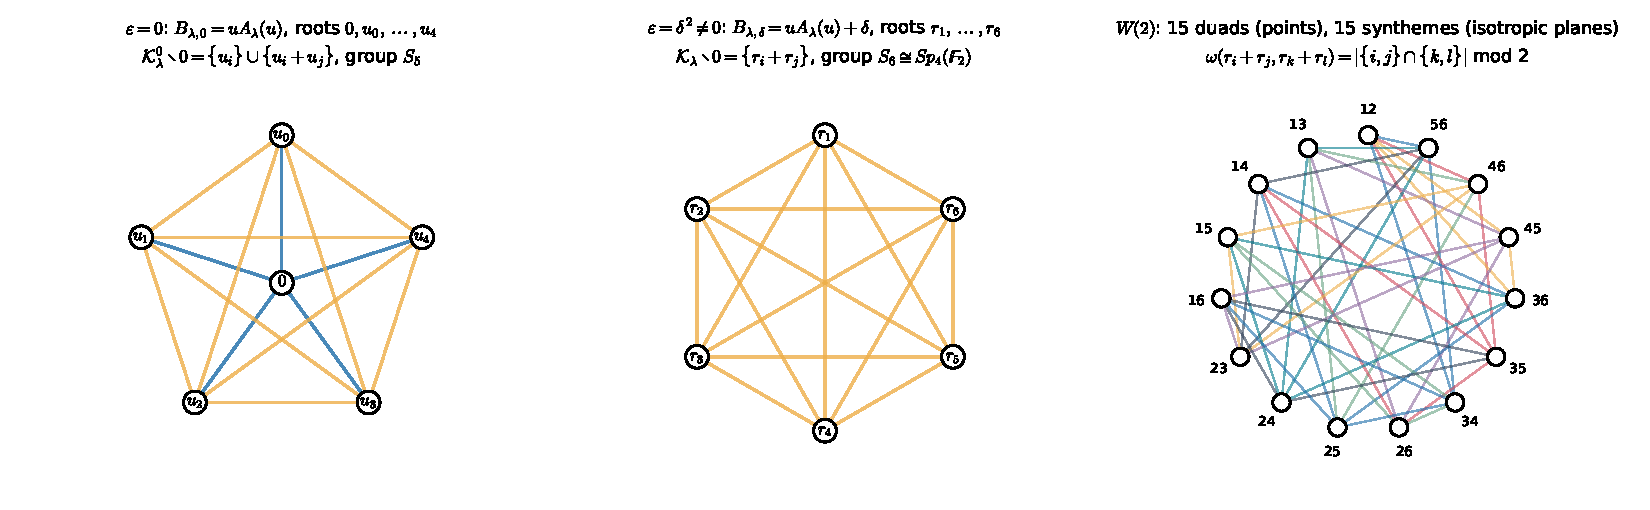
\includegraphics[width=\textwidth]{fig_deformation.pdf}
\caption{Left: the quintic frame ($\eps=0$); the kernel of $L_\lambda$ is $\{0\}\cup\{u_i\}\cup\{u_i+u_j\}$ and the Frobenius acts through $S_5$. Middle: the hexad ($\eps\ne0$); the kernel of $L_\lambda+\eps x^4$ is $\{0\}\cup\{r_i+r_j\}$ and the Frobenius acts through $S_6\cong\Sp_4(\F_2)$. Right: the generalised quadrangle $W(2)$ of duads and synthemes, i.e.\ the points and isotropic lines of $(\Kk_\lambda,\omega)$.}\label{fig:deform}
\end{figure}

\subsection{Canonicity}
A hexad with a given duad set is determined up to translation by an element of the kernel; the normalisation $e_2=0$ (equivalently $b_4=0$ for a monic sextic with $e_1=0$) singles out one translate, because translation by $c$ changes the coefficient of $u^4$ by $\binom62c^2=c^2$. This is how $B_\lambda$ was found: an exhaustive search over the $168$ frames of $\Kk_\lambda$ for the Frobenius-stable translation classes, followed by this normalisation and a linear fit of the coefficients over $\F_q$ as Laurent polynomials in $(\lambda_3,\lambda_5)$ (\S\ref{sec:numerics}). The fit returned $b_3=0$, $b_2=\lambda_3^2/\lambda_5^2$, $b_1=\lambda_5^{-1}$, $b_0=\lambda_5^{-2}$ with a single monomial each, i.e.\ $B_\lambda/\lambda_5^2$, after which Lemmas~\ref{lem:identity}--\ref{lem:pairsum} were found.

\section{The Frobenius classes}\label{sec:galois}

\subsection{Proof of Theorem~\ref{thm:classes}}
Let $\sigma$ be the $q$-Frobenius of $\bar\F$. Since $B_\lambda\in\F_q[u]$, $\sigma$ permutes its roots: $\sigma(r_i)=r_{\pi(i)}$ for a permutation $\pi=\pi_\lambda\in S_6$ whose cycle type is the factorisation type of $B_\lambda$ over $\F_q$. By Theorem~\ref{thm:hexad}(c), $\sigma(r_i+r_j)=r_{\pi(i)}+r_{\pi(j)}$: the action on $\Kk_\lambda\setminus0$ is the action of $\pi$ on duads, and it preserves the alternating form \eqref{eq:omega}. The $11$ conjugacy classes of $S_6$ act on the $15$ duads with the orbit structures listed in Table~\ref{tab:classes}, which are the eleven patterns of Part~II, Table~3 (where they were obtained from the orbits of $\sigma$ on the roots of $L'_\lambda/x$ without knowing the hexad). The fixed vectors of $\sigma^m$ in $\Kk_\lambda$ are $0$ and the duads fixed by $\pi^m$, so $f_m:=\dim\Kk_\lambda^{\sigma^m}=\log_2\bigl(1+\#\{\text{duads fixed by }\pi^m\}\bigr)$, which is computed in Table~\ref{tab:classes}. The field $\F_q(\Kk_\lambda)$ is $\F_{q^{N_0}}$ with $N_0$ the order of $\pi$ acting on duads, which is the order of $\pi$ except for the identity and for the class $2^3$, where $\pi=(12)(34)(56)$ has $\pi^2=1$ but fixes only the three duads $\{12\},\{34\},\{56\}$, so that $N_0=2$. That all eleven classes occur for $q\ge32$ is Table~\ref{tab:counts} (for $q=8$ the classes $1^6$ and $2\,1^4$ have count $0$). \qed

\begin{table}[H]
\centering
\caption{The eleven classes. For each cycle type of $\pi\in S_6$: the orbit lengths on the $15$ duads (= on $\Kk_\lambda\setminus0$), the dimensions $f_m=\dim\Kk_\lambda^{\sigma^m}$ of the fixed spaces of $\sigma^m$ for $m=1,2,3,4,6$ (these are the radical dimensions of the forms $\qq^{(m)}_\lambda$ of \S\ref{sec:witt}), the degree $N_0=[\F_q(\Kk_\lambda):\F_q]$, and the value of $W'/q^7$ found in Part~II (proved here for the class $5\,1$, Theorem~\ref{thm:witt}).}\label{tab:classes}
\small
\begin{tabular}{@{}llcccccccc@{}}
\toprule
class & orbits on duads & $f_1$ & $f_2$ & $f_3$ & $f_4$ & $f_6$ & $N_0$ & $\Kk\subset\F_{q^{12}}$ & $W'/q^7$\\
\midrule
$1^6$ & $(1^{15})$ & 4 & 4 & 4 & 4 & 4 & 1 & yes & $4$\\
$2\,1^4$ & $(1^7,2^4)$ & 3 & 4 & 3 & 4 & 4 & 2 & yes & $0$\\
$2^2\,1^2$ & $(1^3,2^6)$ & 2 & 4 & 2 & 4 & 4 & 2 & yes & $0$\\
$2^3$ & $(1^3,2^6)$ & 2 & 4 & 2 & 4 & 4 & 2 & yes & $4$\\
$3\,1^3$ & $(1^3,3^4)$ & 2 & 2 & 4 & 2 & 4 & 3 & yes & $4$\\
$3^2$ & $(3^5)$ & 0 & 0 & 4 & 0 & 4 & 3 & yes & $4$\\
$3\,2\,1$ & $(1,2,3,3,6)$ & 1 & 2 & 3 & 2 & 4 & 6 & yes & $0$\\
$4\,1^2$ & $(1,2,4,4,4)$ & 1 & 2 & 1 & 4 & 2 & 4 & yes & $2$\\
$4\,2$ & $(1,2,4,4,4)$ & 1 & 2 & 1 & 4 & 2 & 4 & yes & $-2$\\
$5\,1$ & $(5,5,5)$ & 0 & 0 & 0 & 0 & 0 & 5 & no & $-1$\\
$6$ & $(3,6,6)$ & 0 & 0 & 2 & 0 & 4 & 6 & yes & $4$\\
\bottomrule
\end{tabular}
\end{table}

\begin{figure}[H]
\centering
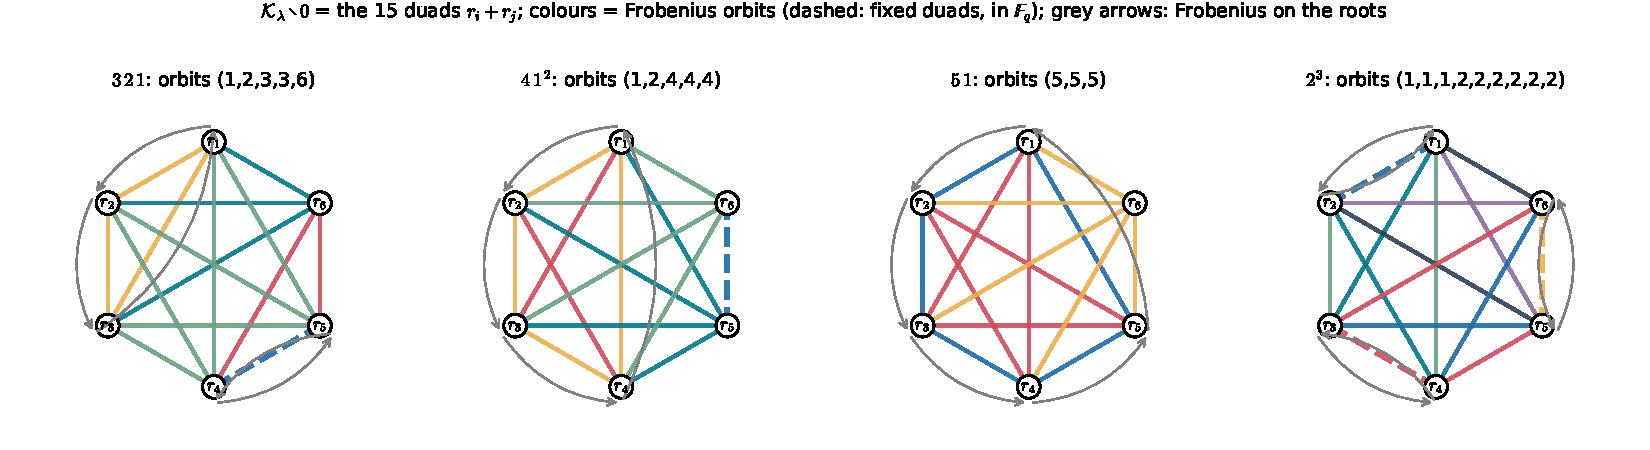
\includegraphics[width=\textwidth]{fig_hexad_orbits.pdf}
\caption{The Frobenius on $\Kk_\lambda\setminus0$ for four classes. Each panel shows the six roots and the fifteen duads coloured by $\sigma$-orbit. The classes $4\,1^2$ and $4\,2$ have the same orbit structure on duads (and so do $2^21^2$ and $2^3$); the hexad distinguishes them, and so do the Witt sums (Theorem~\ref{thm:witt}(d): $W'=+2q^7$ versus $-2q^7$).}\label{fig:orbits}
\end{figure}

\begin{remark}[why there is no parity obstruction]
For the quintic frame of Part~II only three of the seven cycle types of $S_5$ occur, because the radical of the $\F_2$-quadratic form $x\mapsto\Tr_{q/2}(\lambda_5x^5+\lambda_3x^3)$ on $\F_q$ is $\Kk^0_\lambda\cap\F_q=(\Kk^0_\lambda)^\sigma$ and must have dimension $\equiv k\equiv1\pmod 2$. For $L'_\lambda$ the corresponding form on $\F_q$ is $\Z/4$-valued (it is $\qq^{(1)}_\lambda$ of \S\ref{sec:witt}) with a non-alternating polar form, and the radical-parity constraint of alternating forms does not apply; indeed Table~\ref{tab:classes} shows both parities of $f_1$.
\end{remark}

\subsection{Traces on the hexad}
The following lemma, a consequence of Theorem~\ref{thm:moments}, is used repeatedly in Section~\ref{sec:witt}. For a root $r_i$ in a $\pi$-cycle of length $\ell_i$ write $c_i=\sum_{t\in\text{cycle}}r_t\in\F_q$ for the cycle sum.

\begin{lemma}\label{lem:traces}
Let $m$ be a positive integer with $N_0\mid m$, so that $\Kk_\lambda\subset\F_{q^m}$.
\begin{enumerate}[label=\textup{(\roman*)},leftmargin=2em]
\item For every root, $\Tr_{q^m/q}(r_i)=(m/\ell_i)\,c_i$. In particular $\Tr_{q^{12}/q}$ vanishes on $\Kk_\lambda$ unless $N_0=4$, in which case $\Tr_{q^{12}/q}(r_i+r_j)=\tau_0:=r_5+r_6$ (the sum of the two roots outside the $4$-cycle) when exactly one of $i,j$ lies in the $4$-cycle, and $0$ otherwise.
\item If $m$ is even then $\Tr_{q^m/2}$ vanishes on $\Kk_\lambda$.
\item If $N_0\mid4$ then $\Tr_{q^4/q}$ vanishes on $\Kk_\lambda$ unless $N_0=4$, where it is as in \textup{(i)}; and $\Tr_{q/2}(\tau_0)=0$.
\end{enumerate}
\end{lemma}
\begin{proof}
(i) $\Tr_{q^m/q}(r_i)=\sum_{t=0}^{m-1}\sigma^t(r_i)$ runs $m/\ell_i$ times over the cycle. For $m=12$: $12/\ell_i$ is even unless $\ell_i=4$, and for $\ell_i=4$ the cycle sum is $e_1-(r_5+r_6)=\tau_0$. (ii) $\Tr_{q^m/2}(r_i)=\Tr_{q/2}((m/\ell_i)c_i)$; if $m/\ell_i$ is even this is $0$. Otherwise $\ell_i$ is even (as $m$ is), so $\ell_i\in\{2,4,6\}$: for $\ell_i=2$, $c_i=r_i+r_i^q$ with $r_i\in\F_{q^2}\setminus\F_q$; for $\ell_i=4$, $c_i=\tau_0=r_5+r_6$ where $r_5,r_6$ are either both in $\F_q$ or conjugate in $\F_{q^2}$; for $\ell_i=6$, $c_i=e_1=0$. In the first two cases $\Tr_{q/2}(c_i)=0$ by the last assertion of Theorem~\ref{thm:moments}. (iii) is (i) with $12$ replaced by $4$, together with the same trace statement.
\end{proof}

\subsection{Symplectic structures preserved by the Frobenius}\label{subsec:symplectic}
The hexad of $B_\lambda$ is not the only hexad with duad set $\Kk_\lambda\setminus0$ that the Frobenius preserves: by \S\ref{subsec:hexads} the $28$ translation classes of hexads correspond to the $28$ nondegenerate alternating forms on $\Kk_\lambda$, and a class is $\sigma$-stable iff $\sigma\in\Sp(\omega)$ for the corresponding form. With respect to a stable form $\omega$ the element $\sigma$ has an $S_6$-class, which depends on $\omega$. The following proposition explains the counts found by \texttt{hexad\_search.py} (\S\ref{sec:numerics}) and in particular why the orbit structure of $\sigma$ on $\Kk_\lambda\setminus0$ does not determine the class of $B_\lambda$.

\begin{proposition}\label{prop:symplectic}
Let $g\in\GL(V)\cong\GL_4(\F_2)$, let $C$ be its conjugacy class in $\GL(V)$, and let $t$ be a conjugacy class of $S_6\cong\Sp_4(\F_2)$ contained in $C$ (under any of the $28$ identifications $S_6\cong\Sp(V,\omega)$; the image of $t$ in $\GL(V)$ does not depend on $\omega$). Then the number of nondegenerate alternating forms $\omega$ on $V$ with $g\in\Sp(V,\omega)$ and $g$ of type $t$ in $\Sp(V,\omega)\cong S_6$ is $28\,|t|/|C|$. The values are given in Table~\ref{tab:symplectic}.
\end{proposition}
\begin{proof}
Count pairs $(h,\omega)$ with $h\in C$, $h\in\Sp(V,\omega)$ of type $t$. For fixed $\omega$ there are $|t|$ such $h$, so there are $28|t|$ pairs. The number of $\omega$ attached to a given $h\in C$ is constant on $C$, because $\GL(V)$ permutes the forms transitively and $h\mapsto uhu^{-1}$ carries the forms attached to $h$ to those attached to $uhu^{-1}$ (with the same type). Hence each $h\in C$ has $28|t|/|C|$ forms.
\end{proof}

\begin{table}[H]
\centering
\caption{The classes of $\GL_4(\F_2)$ met by $S_6\cong\Sp_4(\F_2)$: for each $S_6$-class $t$, the $\GL_4(\F_2)$-class $C\supset t$ described by the Jordan or rational canonical form of its elements and its size $|C|=|\GL_4(\F_2)|/|\mathrm{Cent}(g)|$, and the number $28|t|/|C|$ of $g$-stable symplectic forms in which $g$ has type $t$ (Proposition~\ref{prop:symplectic}). The last column is the number of Frobenius-stable translation classes of hexads found by \texttt{hexad\_search.py} for every pair at $q=8$ and $q=32$, by canonical class, with the types of $\sigma$ in those classes (the class $5\,1$ was not searched since $\Kk_\lambda\not\subset\F_{q^{12}}$).}\label{tab:symplectic}
\small
\begin{tabular}{@{}llllll@{}}
\toprule
$t$ & $|t|$ & $C$ (canonical form, $f_1$) & $|C|$ & $28|t|/|C|$ & found\\
\midrule
$1^6$ & 1 & identity & 1 & 28 & 28\\
$2\,1^4$ & 15 & transvection $J_2\oplus J_1^2$, $f_1=3$ & 105 & 4 & 4\\
$2^2\,1^2$ & 45 & $J_2\oplus J_2$, $f_1=2$ & 210 & 6 & \multirow{2}{*}{$8=6+2$}\\
$2^3$ & 15 & $J_2\oplus J_2$, $f_1=2$ & 210 & 2 & \\
$3\,1^3$ & 40 & $\F_4$-scalar on a plane, $f_1=2$ & 1120 & 1 & 1\\
$3^2$ & 40 & $\F_4$-scalar on $V\cong\F_4^2$, $f_1=0$ & 112 & 10 & 10\\
$3\,2\,1$ & 120 & order $6$, $f_1=1$ & 3360 & 1 & 1\\
$4\,1^2$ & 90 & regular unipotent $J_4$, $f_1=1$ & 2520 & 1 & \multirow{2}{*}{$2=1+1$}\\
$4\,2$ & 90 & regular unipotent $J_4$, $f_1=1$ & 2520 & 1 & \\
$5\,1$ & 144 & order $5$, $f_1=0$ & 1344 & 3 & --\\
$6$ & 120 & order $6$, $f_1=0$ & 1680 & 2 & 2\\
\bottomrule
\end{tabular}
\end{table}

\begin{remark}
The class sizes are $|\GL_4(\F_2)|=20160$ divided by the centraliser orders $20160$, $192$, $96$, $18$, $180$, $6$, $8$, $15$, $12$; e.g.\ the centraliser of $J_2\oplus J_2$ is $\GL_2(\F_2[\epsilon]/\epsilon^2)$ of order $6\cdot16=96$, that of a regular unipotent is the group of units of $\F_2[g]$, of order $8$, and the elements of order $3$ without fixed vectors are the $\F_4$-scalars of the $112=|\GL_4(\F_2)|/|\GL_2(\F_4)|$ structures of $\F_4$-space on $V$. Two consequences: (i) a Frobenius of class $2^21^2$ or $2^3$ is of type $2^21^2$ for six of its eight stable forms and of type $2^3$ for the other two; a Frobenius of order $4$ is of type $4\,1^2$ for one of its two stable forms and of type $4\,2$ for the other. The value of $W'$ follows the type with respect to the \emph{canonical} form, the one defined by $B_\lambda$ (Theorem~\ref{thm:witt}(d): $+2q^7$ for $4\,1^2$, $-2q^7$ for $4\,2$); so the canonical symplectic structure carries arithmetic information that the $\F_2[\sigma]$-module $\Kk_\lambda$ alone does not. (ii) A Frobenius of class $5\,1$ preserves three symplectic forms, and is a $5$-cycle for all of them; here $\Kk_\lambda\subset\F_{q^5}$ and the three stable hexads live in $\F_{q^5}$, outside the field $\F_{q^{12}}$ in which the search was carried out.
\end{remark}

\section{Counting}\label{sec:counting}

\subsection{The family}
By Lemma~\ref{lem:separable} the map $(\lambda_3,\lambda_5)\mapsto\lambda_5^{-2}B_\lambda$ is a bijection from $\F_q\times\F_q^\times$ onto the set of monic sextics
\begin{equation}\label{eq:family}
F_{a,b}(u)=u^6+au^2+bu+b^2,\qquad a\in\F_q,\ b\in\F_q^\times,\qquad a=\lambda_3^2/\lambda_5^2,\ b=\lambda_5^{-1},
\end{equation}
i.e.\ onto the monic sextics with $e_1=e_2=e_3=0$ and $e_6=e_5^2\ne0$. The sub-family $a=0$ ($\lambda_3=0$) is $u^6+bu+b^2$. With $u=bw$, $F_{a,b}(bw)=b^2\bigl(b^4w^6+aw^2+w+1\bigr)$, and with $u=1/v$, $v^6F_{a,b}(1/v)=b^2v^6+bv^5+av^4+1$, so that after scaling the family is also $v^6+v^5+a'v^4+c$ with $c=b^4$, $a'=a/b^2$.

\subsection{Proof of Theorem~\ref{thm:moments}}
\emph{Rational roots.} A root $u_0\in\F_q$ of $F_{a,b}$ is nonzero ($F(0)=b^2$), and for given $u_0\in\F_q^\times$ and $b\in\F_q^\times$ the equation $F_{a,b}(u_0)=0$ is linear in $a$ with the unique solution $a=(u_0^6+bu_0+b^2)/u_0^2\in\F_q$. Hence $\sum_{(a,b)}N_1=(q-1)^2$.

\emph{Pairs of rational roots.} Let $r\ne s$ in $\F_q^\times$ be roots of $F_{a,b}$. Then $s^2F(r)+r^2F(s)=r^2s^2(r^4+s^4)+b\,rs(r+s)+b^2(r+s)^2=0$, and dividing by $(r+s)^2$,
\[
b^2+\frac{rs}{r+s}\,b+r^2s^2(r+s)^2=0 .
\]
Writing $b=\frac{rs}{r+s}\,z$ this is $z^2+z=(r+s)^4$, which has two solutions $z\in\F_q$ iff $\Tr_{q/2}(r+s)=\Tr_{q/2}((r+s)^4)=0$ and none otherwise; the solutions $b$ are nonzero, and $a$ is then determined. This proves the last assertion of the theorem for rational pairs, and shows that the number of triples $(a,b;r,s)$ with $r\ne s$ rational roots is $2\cdot\#\{(r,s)\in(\F_q^\times)^2:r\ne s,\ \Tr(r+s)=0\}$. For fixed $r\ne0$ the number of $s\ne0$ with $\Tr s=\Tr r$ is $q/2-1$ if $\Tr r=0$ and $q/2$ if $\Tr r=1$, and we must remove $s=r$: the count is $(q/2-1)^2+(q/2)^2-(q-1)=q^2/2-2q+2$, and twice this is $(q-2)^2$.

\emph{Roots in $\F_{q^2}\setminus\F_q$.} Let $u_0\in\F_{q^2}\setminus\F_q$, $\bar u_0=u_0^q$, $s=u_0+\bar u_0\ne0$, $n=u_0\bar u_0$. For given $b\in\F_q^\times$ the value $a=u_0^4+b/u_0+b^2/u_0^2$ lies in $\F_q$ iff it equals its conjugate, i.e.\ iff $s^4+bs/n+b^2s^2/n^2=0$, i.e.\ $s^3n^2+bn+b^2s=0$. With $n=(b/s^3)m$ this becomes $m^2+m=s^4$, solvable iff $\Tr_{q/2}(s)=0$, with solutions $m,m+1$; this is the last assertion of the theorem for conjugate pairs. The pair $(s,n)$ corresponds to a conjugate pair $u_0,\bar u_0\notin\F_q$ iff $u^2+su+n$ is irreducible, i.e.\ $\Tr_{q/2}(n/s^2)=\Tr_{q/2}(bm/s^5)=1$. Hence the number of pairs $(b,u_0)$ is
\begin{multline*}
\sum_{\substack{s\ne0\\ \Tr s=0}}\ \sum_{b\ne0}\ 2\Bigl(\bigl[\Tr(bm/s^5)=1\bigr]+\bigl[\Tr(b(m+1)/s^5)=1\bigr]\Bigr)\\
=\sum_{\substack{s\ne0\\ \Tr s=0}}2\Bigl(\frac q2+\frac q2\Bigr)=2q\Bigl(\frac q2-1\Bigr)=q(q-2),
\end{multline*}
using that $b\mapsto\Tr(b\gamma)$ takes the value $1$ exactly $q/2$ times for $\gamma\ne0$, that $m,m+1\ne0$ because $m^2+m=s^4\ne0$, and that each $(s,n)$ accounts for the two roots $u_0,\bar u_0$. Each such pair gives a unique $a$. \qed

\begin{corollary}\label{cor:relations}
Let $n_C$ be the number of $(\lambda_3,\lambda_5)\in\F_q\times\F_q^\times$ whose sextic has class $C$, and let $f_C$, $f_C^{(2)}$ be the numbers of fixed points of $\pi$ and $\pi^2$ on $\{1,\dots,6\}$ for $\pi\in C$. Then
\begin{gather*}
\sum_Cn_C=q(q-1),\qquad \sum_Cn_Cf_C=(q-1)^2,\\
\sum_Cn_Cf_C(f_C-1)=(q-2)^2,\qquad \sum_Cn_C\bigl(f_C^{(2)}-f_C\bigr)=q(q-2).
\end{gather*}
\end{corollary}

\subsection{The class counts}
\begin{table}[H]
\centering
\caption{Number of $(\lambda_3,\lambda_5)\in\F_q\times\F_q^\times$ with $B_\lambda$ of a given factorisation type over $\F_q$, $k$ odd: the polynomials of Part~II, Table~3 (mixed pairs, $\lambda_3\ne0$) and of Part~II, Lemma~6.17 and Proposition~6.8 (pure quintic pairs, $\lambda_3=0$), verified for all pairs and all $q\in\{8,32,128,512\}$ (\texttt{sextic\_types.py}). The last column is the proportion of the class in $S_6$.}\label{tab:counts}
\small
\begin{tabular}{@{}llll@{}}
\toprule
class & $\lambda_3\ne0$ & $\lambda_3=0$ & $|C|/720$\\
\midrule
$1^6$ & $(q-2)(q-8)/720$ & $0$ & $1/720$\\
$2\,1^4$ & $(q-2)(q-8)/48$ & $0$ & $1/48$\\
$2^2\,1^2$ & $q(q-2)/16$ & $0$ & $1/16$\\
$2^3$ & $(q-2)(q-8)/48$ & $(q-2)/6$ & $1/48$\\
$3\,1^3$ & $(q+1)(q-2)/18$ & $0$ & $1/18$\\
$3^2$ & $(q+1)(q-2)/18$ & $0$ & $1/18$\\
$3\,2\,1$ & $(q+1)(q-2)/6$ & $0$ & $1/6$\\
$4\,1^2$ & $(q-2)(q-4)/8$ & $(q-2)/2$ & $1/8$\\
$4\,2$ & $q(q-2)/8$ & $0$ & $1/8$\\
$5\,1$ & $(q^2+1)/5$ & $0$ & $1/5$\\
$6$ & $(q+1)(q-2)/6$ & $(q+1)/3$ & $1/6$\\
\bottomrule
\end{tabular}
\end{table}

\begin{proposition}\label{prop:countsverified}
For $q\in\{8,32,128,512\}$ the numbers of $(\lambda_3,\lambda_5)$ with $B_\lambda$ of each factorisation type are exactly the entries of Table~\ref{tab:counts}. The entries satisfy the four identities of Corollary~\ref{cor:relations} as polynomial identities in $q$. The column $\lambda_3=0$ is a theorem for all odd $k$.
\end{proposition}
\begin{proof}
The verification factors the $q(q-1)$ sextics over $\F_q$ by computing $\gcd(B,u^{q^m}-u)$ for $m\le6$ ($q=512$: $261\,632$ sextics). The identities are checked by expanding; e.g.\ $\sum n_Cf_C=6\frac{(q-2)(q-8)}{720}+4\frac{(q-2)(q-8)}{48}+2\frac{q(q-2)}{16}+3\frac{(q+1)(q-2)}{18}+\frac{(q+1)(q-2)}6+2\frac{(q-2)(q-4)}8+\frac{q^2+1}5+2\cdot\frac{q-2}2=(q-1)^2$.

For $\lambda_3=0$, Part~II, Lemma~6.17, shows that $\Kk_{(0,\lambda_5)}$ is obtained from the quintic frame of the Gold quintic $v^5+v+\lambda_5^2$ by extracting cube roots, with orbit structure on $\Kk\setminus0$ equal to $(1,2,4,4,4)$, $(1^3,2^6)$, $(3,6,6)$ for the quintic types $(1,4)$, $(1,1,1,2)$, $(2,3)$, whose numbers are $(q-2)/2$, $(q-2)/6$, $(q+1)/3$ by Part~II, Proposition~6.8. By Table~\ref{tab:classes} the sextic classes with these orbit structures are $\{4\,1^2,4\,2\}$, $\{2^21^2,2^3\}$ and $\{6\}$ respectively. The first moment decides between the alternatives: the number of rational roots of $u^6+bu+b^2$ summed over $b\in\F_q^\times$ is, by the computation above with $a=0$ (for $u_0\in\F_q^\times$ the equation $b^2+u_0b+u_0^6=0$, i.e.\ $z^2+z=u_0^4$ with $b=u_0z$, has two solutions iff $\Tr u_0=0$), equal to $2(q/2-1)=q-2$. The classes $4\,1^2$ and $2^21^2$ have two rational roots each, $4\,2$ and $2^3$ none; so $q-2=2\alpha\frac{q-2}2+2\beta\frac{q-2}6$ with $\alpha,\beta\in\{0,1\}$ indicating the choices $4\,1^2$ and $2^21^2$, whose only solution is $\alpha=1$, $\beta=0$.
\end{proof}

\begin{conjecture}\label{conj:counts}
Table~\ref{tab:counts} holds for all odd $k$.
\end{conjecture}

\begin{figure}[H]
\centering
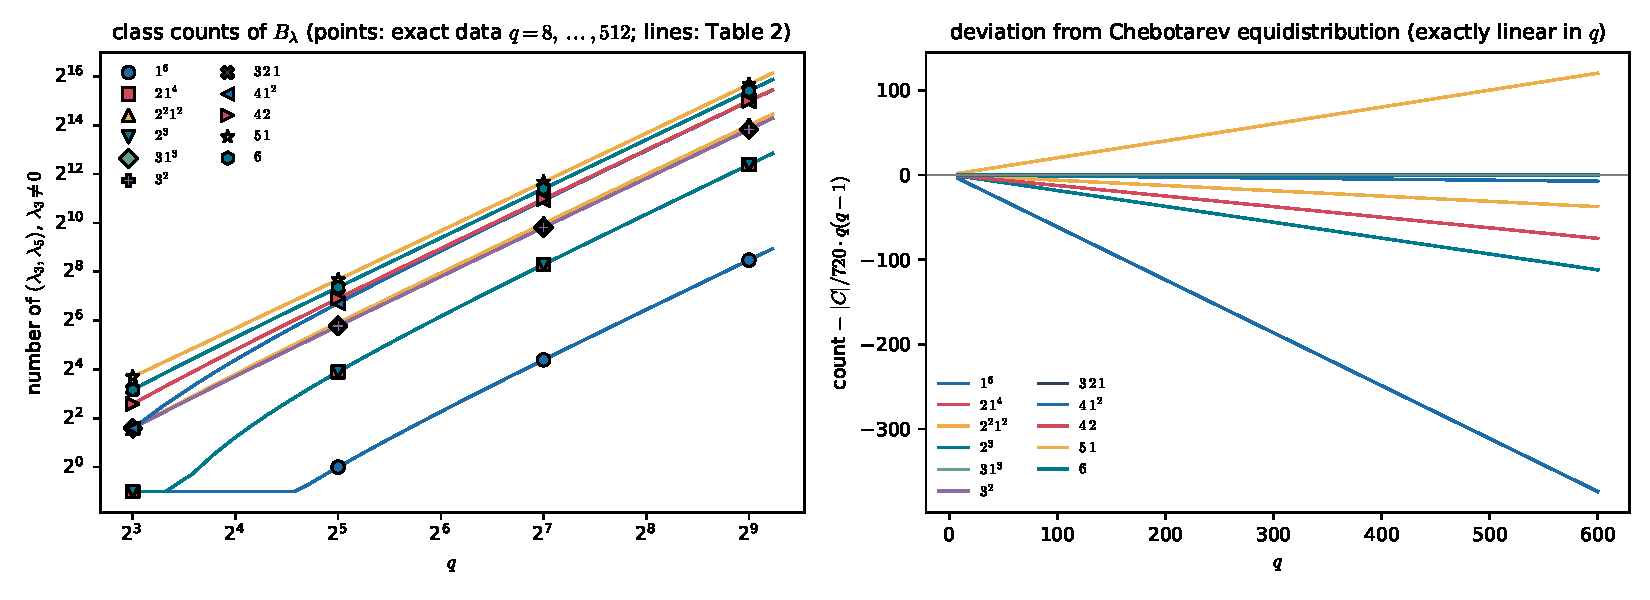
\includegraphics[width=\textwidth]{fig_class_counts.pdf}
\caption{Left: the class counts of $B_\lambda$ for $\lambda_3\ne0$ (points: exact data for $q=8,32,128,512$; lines: the polynomials of Table~\ref{tab:counts}; counts equal to $0$ are drawn at $2^{-1}$). Right: the deviation of each count from the Chebotarev proportion $|C|/720\cdot q(q-1)$ is exactly linear in $q$.}\label{fig:counts}
\end{figure}

\begin{remark}
The leading coefficients are the class proportions of $S_6$: the family is equidistributed in the sense of Chebotarev, as expected since its geometric monodromy group is $S_6$ ($S_6$ is the only subgroup of $S_6$ containing a $5$-cycle, a $6$-cycle and a transposition). What is remarkable is the absence of any error term: the counts are polynomials with the same value for every odd $k$. For the quintic $v^5+v+c$ this exactness was proved in Part~II by counting roots in $\F_q$ and $\F_{q^2}$ (two linear relations suffice for three classes). For the sextic the analogous relations are the four of Corollary~\ref{cor:relations}, which do not determine eleven unknowns; the higher moments ($N_m$ for $m\le6$ and the second moments over $\F_{q^2},\F_{q^3}$) are counts of points on explicit curves over $\F_q$, e.g.\ $N_3$ is the number of $(w,a')\in\F_{q^3}\times\F_q$ with $w^4(w^2+w+a')\in\F_q$ in the normalisation $v^6+v^5+a'v^4+c$, and the exactness of Table~\ref{tab:counts} says that all these curves have polynomial point counts. We leave this as Open Problem~\ref{op:counts}.
\end{remark}

\section{The Witt sums}\label{sec:witt}

\subsection{Two parametrisations of the order-four characters}
\begin{lemma}\label{lem:SpSpp}
Let $\tau=\Tr_{q^{12}/q}$ and let $S'(\lambda)$, $\Spp(\lambda)$ be as in \eqref{eq:XW}, \eqref{eq:Spp}. For $x\in\F_{q^{12}}$,
\[
\mathsf T_{12k}(x)=\Tr_{q/2}(\tau x)+2\bigl(\Tr_{q/2}e_2(x)+e_2^{{\rm abs},\F_q}(\tau x)\bigr),
\]
where $e_2(x)$ is relative to $\F_q$ (twelve conjugates) and $e_2^{{\rm abs},\F_q}(y)=\sum_{0\le i<j<k}y^{2^i+2^j}$ for $y\in\F_q$. Consequently $S'(\lambda)$ and $\Spp(\lambda)$ have the same restriction to $\{\tau x=0\}$, and
\[
\sum_{\lambda_1}S'(\lambda)=\sum_{\lambda_1}\Spp(\lambda)=q\sum_{\tau x=0}(-1)^{\Tr(\lambda_5x^5+\lambda_3x^3)+\Tr_{q/2}e_2(x)}=W'(\lambda_3,\lambda_5),
\]
but $S'(\lambda)\ne\Spp(\lambda)$ in general.
\end{lemma}
\begin{proof}
Transitivity of the Witt trace: $\Tr_{W_2(\F_{q^{12}})/\Z/4}[x]=\Tr_{W_2(\F_q)/\Z/4}\bigl(\Tr_{W_2(\F_{q^{12}})/W_2(\F_q)}[x]\bigr)$, and the inner trace is the Witt sum of the twelve Teichm\"uller lifts of the conjugates, $(\tau x,e_2(x))$; then $(y_0,y_1)=[y_0]+(0,y_1)$ and $\Tr_{W_2(\F_q)/\Z/4}(0,y_1)=2\Tr_{q/2}y_1$. The sum over $\lambda_1$ of $(-1)^{\Tr(\lambda_1x)}$ is $q[\tau x=0]$ in both parametrisations.
\end{proof}

Thus $W'$ does not depend on which of the two families of order-$4$ characters is used, but only $\Spp$ has an $L$-function: the sheaf $\mathcal L_{\psi_4}(x,f_\lambda(x))$ on $\A^1_{\F_q}$, $f_\lambda=\lambda_5x^5+\lambda_3x^3+\lambda_1x$, for the character $\psi_4(a_0+2a_1)=i^{a_0+2a_1}$ of $\Z/4=W_2(\F_2)$, has trace function $x\mapsto i^{\mathsf T_{mk}(x)+2\Tr_{q^m/2}f_\lambda(x)}$ at $x\in\F_{q^m}$ (the Witt vector $(x,f_\lambda(x))=[x]+Vf_\lambda(x)$), is lisse of rank one and pure of weight $0$ on $\A^1$, and has Swan conductor $\max(2\deg x,\deg f_\lambda)=5$ at infinity when $\lambda_5\ne0$ \cite{Brylinski,Katz}. By the Grothendieck--Ogg--Shafarevich formula $\chi_c(\A^1_{\bar\F},\mathcal L)=1-5=-4$, and $H^0_c=H^2_c=0$ as the sheaf is nontrivial and lisse on an affine curve; so $H^1_c$ has rank $4$ with Frobenius eigenvalues $\omega_1,\dots,\omega_4$, and by Deligne \cite{Deligne} $|\omega_j|\le\sqrt q$ for every complex embedding. Writing
\begin{equation}\label{eq:sm}
s_m(\lambda):=\sum_{x\in\F_{q^m}}i^{\qq^{(m)}_\lambda(x)},\qquad \qq^{(m)}_\lambda(x):=\mathsf T_{mk}(x)+2\Tr_{q^m/2}f_\lambda(x),
\end{equation}
the Lefschetz trace formula gives
\begin{equation}\label{eq:Lpoly}
s_m(\lambda)=-\sum_{j=1}^4\omega_j^m\quad(m\ge1),\qquad \Spp(\lambda)=s_{12}(\lambda).
\end{equation}

\subsection{The \texorpdfstring{$\Z/4$}{Z/4}-forms and their radicals}
\begin{proposition}\label{prop:Z4form}
For every $m\ge1$, $\qq^{(m)}_\lambda$ is a $\Z/4$-valued quadratic form on $\F_{q^m}$ with polar form $b^{(m)}_\lambda(x,y)=\Tr_{q^m/2}\bigl(x\,T'_\lambda(y)\bigr)$, radical $\Rr^{(m)}_\lambda=\Kk_\lambda\cap\F_{q^m}=\Kk_\lambda^{\sigma^m}$ of dimension $f_m$ (Table~\ref{tab:classes}), and characteristic element any element of $T_\lambda'^{-1}(1)\cap\F_{q^m}$ when this set is nonempty. Consequently
\[
s_m(\lambda)\in\{0\}\cup 2^{(mk+f_m)/2}\mu_8,\qquad s_m(\lambda)\ne0\iff\qq^{(m)}_\lambda|_{\Kk_\lambda\cap\F_{q^m}}=0 .
\]
On the radical, $\qq^{(m)}_\lambda(x)=\mathsf T_{mk}(x)+2\Tr_{q^m/2}(\lambda_5x^5+\lambda_3x^3)+2\Tr_{q/2}\bigl(\lambda_1\Tr_{q^m/q}x\bigr)$ is additive and $\sigma$-invariant.
\end{proposition}
\begin{proof}
By \eqref{eq:Tpolar} the polar form of $\mathsf T_{mk}$ is $2\Tr_{q^m/2}(xy)$; that of $2\Tr_{q^m/2}f_\lambda$ is $2\Tr_{q^m/2}(xT_\lambda(y))$ (the polar form of the $\F_2$-form $\Tr(\lambda_5x^5+\lambda_3x^3)$ is $\Tr(y(D_\lambda+D_\lambda^*)(x))$, and the linear term has none). Adding, $b^{(m)}_\lambda(x,y)=\Tr_{q^m/2}(x(T_\lambda+1)(y))$; note that $T'_\lambda$ maps $\F_{q^m}$ to itself. The radical is $\ker T'_\lambda\cap\F_{q^m}$ by nondegeneracy of the trace form. Next $b(x,x)=\Tr_{q^m/2}(xT'_\lambda(x))=\Tr_{q^m/2}(x^2)+\Tr_{q^m/2}(\lambda_5x^5+\lambda_3x^3)+\Tr_{q^m/2}\bigl(x(\lambda_3x)^{1/2}+x(\lambda_5x)^{1/4}\bigr)=\Tr_{q^m/2}(x)$, because $\Tr(x(\lambda_3x)^{1/2})=\Tr((\lambda_3x^3)^{1/2})=\Tr(\lambda_3x^3)$ and similarly for the quintic term; and $\Tr(x)=\Tr(xT'_\lambda(w))$ for all $x$ iff $T'_\lambda(w)=1$. The rest is \eqref{eq:gaussmod} and $\dim\Rr^{(m)}=f_m$ (Theorem~\ref{thm:classes}).
\end{proof}

\subsection{The multiplicity formula along towers}
\begin{lemma}\label{lem:multiplicity}
Let $m\mid M$ and $x\in\F_{q^m}\subset\F_{q^M}$. Then, in $\Z/4$,
\[
\qq^{(M)}_\lambda(x)=\frac Mm\cdot\qq^{(m)}_\lambda(x)=
\begin{cases}
\qq^{(m)}_\lambda(x)&M/m\equiv1\pmod4,\\
2\Tr_{q^m/2}(x)&M/m\equiv2\pmod4,\\
\qq^{(m)}_\lambda(x)+2\Tr_{q^m/2}(x)&M/m\equiv3\pmod4,\\
0&M/m\equiv0\pmod4.
\end{cases}
\]
In particular, for $M=12$: $\qq^{(12)}_\lambda$ vanishes identically on $\F_q$ and on $\F_{q^3}$, equals $2\Tr_{q^2/2}$ on $\F_{q^2}$ and $2\Tr_{q^6/2}$ on $\F_{q^6}$, and equals $\qq^{(4)}_\lambda+2\Tr_{q^4/2}$ on $\F_{q^4}$.
\end{lemma}
\begin{proof}
$\Tr_{W_2(\F_{q^M})/W_2(\F_{q^m})}[x]$ is the sum of $M/m$ copies of $[x]$, i.e.\ $(M/m)\cdot[x]$ with $M/m\in\Z/4=W_2(\F_2)$ acting through the ring structure; the trace $W_2(\F_{q^m})\to\Z/4$ is $\Z/4$-linear, so $\mathsf T_{Mk}(x)=(M/m)\mathsf T_{mk}(x)$. Also $2\Tr_{q^M/2}f_\lambda(x)=2(M/m)\Tr_{q^m/2}f_\lambda(x)$. The case distinction uses $2v=2(v\bmod2)$ and $3v=v+2(v\bmod2)$ in $\Z/4$ together with $\qq^{(m)}_\lambda(x)\equiv\Tr_{q^m/2}(x)\pmod2$.
\end{proof}

\subsection{Integrality and the shift calculus}
\begin{lemma}[shifts]\label{lem:wittshift}
Let $c\in\F_{q^m}$ with $T'_\lambda(c)=a\in\F_q$. Then, with $\lambda_3,\lambda_5$ fixed,
\[
s_m(\lambda_1)=i^{\qq^{(m)}_\lambda(c)}\,s_m(\lambda_1+a).
\]
For $m=12$ and $c\in\F_q$ the phase is trivial, so $\Spp$ is constant on cosets of $T'_\lambda(\F_q)$ in $\F_q$.
\end{lemma}
\begin{proof}
\eqref{eq:shift} with $2b^{(m)}(x,c)=2\Tr_{q^m/2}(xT'_\lambda(c))=2\Tr_{q^m/2}(ax)$, which is the change $\lambda_1\mapsto\lambda_1+a$ in $2\Tr f_\lambda$. For $c\in\F_q$, $\qq^{(12)}_\lambda(c)=0$ by Lemma~\ref{lem:multiplicity}.
\end{proof}

\begin{proposition}[integrality]\label{prop:real}
For all $\lambda$, with $\lambda_3,\lambda_5$ fixed: $\overline{\Spp(\lambda_1)}=\Spp(\lambda_1+1)=\Spp(\lambda_1)$. Hence $\Spp(\lambda)\in\Z$, and more precisely $\Spp(\lambda)\in\{0,\pm4q^6\}$ if $\Kk_\lambda\subset\F_{q^{12}}$ and $\Spp(\lambda)=\pm q^6$ otherwise.
\end{proposition}
\begin{proof}
Complex conjugation replaces $\qq$ by $-\qq=\qq+2(\qq\bmod2)=\qq+2\Tr_{q^{12}/2}(x)$, which is $\qq_{\lambda_1+1}$: this is the first equality. For the second, pick a root $r$ of $B_\lambda$ in $\F_{q^{12}}$ with $\qq^{(12)}_\lambda(r)=0$; such a root exists: if $r$ lies in a $\pi$-cycle of length $\ell\in\{1,3\}$ then $r\in\F_{q^\ell}$ and $\qq^{(12)}(r)=(12/\ell)\qq^{(\ell)}(r)=0$ by Lemma~\ref{lem:multiplicity}; if $\ell\in\{2,6\}$ then $\qq^{(12)}(r)=2\Tr_{q^\ell/2}(r)=2\Tr_{q/2}(c)$ with $c=\Tr_{q^\ell/q}(r)$ the cycle sum, which has trace $0$ by Theorem~\ref{thm:moments} ($\ell=2$) or vanishes because $c=e_1=0$ ($\ell=6$); and every class has a root with $\ell\in\{1,2,3,6\}$ (in the classes $4\,1^2$, $4\,2$ take $r_5$, in the class $5\,1$ take the rational root). Since $T'_\lambda(r)=1$, Lemma~\ref{lem:wittshift} gives $\Spp(\lambda_1)=i^{0}\Spp(\lambda_1+1)$. Thus $\Spp(\lambda)$ is real, and by Proposition~\ref{prop:Z4form} it is $0$ or $2^{(12k+f_{12})/2}$ times an $8$th root of unity, with $f_{12}=4$ if $\Kk_\lambda\subset\F_{q^{12}}$ and $f_{12}=0$ otherwise; a real element of $\mu_8$ is $\pm1$. In the class $5\,1$ the radical is $0$, so $\Spp\ne0$.
\end{proof}

\subsection{The eigenvalues are roots of unity}
\begin{theorem}\label{thm:rootsofunity}
Let $N_0=[\F_q(\Kk_\lambda):\F_q]$. Then $s_{4N_0}(\lambda)\ne0$, $|s_{4N_0}(\lambda)|=4q^{2N_0}$, and
\[
\omega_1^{4N_0}=\omega_2^{4N_0}=\omega_3^{4N_0}=\omega_4^{4N_0}=-\tfrac14s_{4N_0}(\lambda)=q^{2N_0}\nu,\qquad \nu\in\mu_8 .
\]
In particular $|\omega_j|=\sqrt q$ and $\zeta_j:=\omega_j/\sqrt q$ satisfies $\zeta_j^{32N_0}=1$.
\end{theorem}
\begin{proof}
$\Kk_\lambda\subset\F_{q^{N_0}}\subset\F_{q^{4N_0}}$, so the radical of $\qq^{(4N_0)}_\lambda$ is all of $\Kk_\lambda$ (dimension $4$), and $\qq^{(4N_0)}_\lambda$ vanishes on $\F_{q^{N_0}}$ by Lemma~\ref{lem:multiplicity} ($M/m=4$). Hence $s_{4N_0}=2^{(4N_0k+4)/2}\zeta_8^b=4q^{2N_0}\zeta_8^b$ by \eqref{eq:gaussmod}. Now $-s_{4N_0}=\sum_j\omega_j^{4N_0}$ is a sum of four complex numbers of modulus $\le q^{2N_0}$ (Deligne) whose modulus is $4q^{2N_0}$; so all four are equal to $-s_{4N_0}/4$ and have modulus $q^{2N_0}$.
\end{proof}

\begin{corollary}\label{cor:Lprinciple}
The four Gauss sums $s_1,\dots,s_4$ over $\F_q,\dots,\F_{q^4}$ determine the $\omega_j$ (Newton's identities) and hence $\Spp(\lambda)=-\sum_j\omega_j^{12}$. If $\Kk_\lambda\subset\F_{q^{12}}$ then $\Spp(\lambda)\ne0$ iff $\omega_1^{12}=\dots=\omega_4^{12}=-\Spp(\lambda)/4=\mp q^6$, i.e.\ iff $\zeta_j^{12}=\mp1$ for all $j$, where $\Spp(\lambda)=\pm4q^6$; in that case the $\zeta_j$ are $24$th roots of unity.
\end{corollary}
\begin{proof}
The first statement is \eqref{eq:Lpoly}. If $\Spp=\pm4q^6$ then $|\sum\omega_j^{12}|=4q^6$ with $|\omega_j^{12}|=q^6$ forces equality of the four terms; conversely if all $\omega_j^{12}$ are equal to $\mp q^6$ then $\Spp=\pm4q^6$.
\end{proof}

\begin{remark}
Thus, when $\Kk_\lambda\subset\F_{q^{12}}$, the sign of a nonzero $\Spp(\lambda)$ is the statement that the geometric Frobenius over $\F_{q^{12}}$ acts on $H^1_c$ as the scalar $-q^6$ ($\Spp=+4q^6$) or $+q^6$ ($\Spp=-4q^6$), and $\Spp(\lambda)=0$ means that $\omega_j^{12}=q^6$ for two $j$ and $-q^6$ for the other two. This is the Witt-sheaf analogue of the supersingularity statement $\mathrm{Frob}^{N}=\pm q^{N/2}$ for the Artin--Schreier curves of Part~II, and all three cases occur (Table~\ref{tab:eigen}, Figure~\ref{fig:eigen}).
\end{remark}

\subsection{The class of 5-cycles}
\begin{theorem}\label{thm:fivecycle}
Suppose $B_\lambda$ has an irreducible quintic factor over $\F_q$ ($k$ odd). Then:
\begin{enumerate}[label=\textup{(\roman*)},leftmargin=2em]
\item the normalised eigenvalues $\zeta_j=\omega_j/\sqrt q$ are distinct and $\zeta_j^5$ is the same for all $j$;
\item $s_1(\lambda)=\eta\sqrt q$ with $\eta$ a primitive $8$th root of unity, and $\{\zeta_1,\dots,\zeta_4\}=\{\eta\zeta_5^c:c=1,2,3,4\}$;
\item $\prod_j(1-\omega_jT)=\dfrac{1-\eta^5q^{5/2}T^5}{1-\eta q^{1/2}T}=1+s_1T+s_1^2T^2+s_1^3T^3+s_1^4T^4$, and $s_m(\lambda)=s_1(\lambda)^m$ for all $m$ with $5\nmid m$, $s_m(\lambda)=-4s_1(\lambda)^m$ for $5\mid m$;
\item $\Spp(\lambda_1,\lambda_3,\lambda_5)=q^6\eta^4=-q^6$ for every $\lambda_1\in\F_q$, and $W'(\lambda_3,\lambda_5)=-q^7$.
\end{enumerate}
\end{theorem}
\begin{proof}
Here $N_0=5$, the orbits of $\sigma$ on the duads are $(5,5,5)$, and $\pi^m$ is again a $5$-cycle for $5\nmid m$; so $f_m=0$ for $5\nmid m$ and $f_m=4$ for $5\mid m$ (Theorem~\ref{thm:classes}). By Proposition~\ref{prop:Z4form}, $|s_m|=q^{m/2}$ for $5\nmid m$ (a Gauss sum with trivial radical is nonzero) and $|s_m|\in\{0,4q^{m/2}\}$ for $5\mid m$. Put $p_m=\sum_j\zeta_j^m=-s_m/q^{m/2}$. By Theorem~\ref{thm:rootsofunity} the $\zeta_j$ are roots of unity, of order dividing some $N$ which we may take divisible by $5$. Averaging over a period,
\[
\frac1N\sum_{m=1}^N|p_m|^2=\sum_{j,l}\frac1N\sum_{m=1}^N(\zeta_j\bar\zeta_l)^m=\#\{(j,l):\zeta_j=\zeta_l\}\ \ge\ 4 ,
\]
while $|p_m|^2=1$ for the $4N/5$ indices with $5\nmid m$ and $|p_m|^2\le16$ for the $N/5$ others, so the average is $\le\frac45+\frac{16}5=4$. Hence equality holds throughout: the $\zeta_j$ are distinct, and $|p_m|=4$ for every $m\equiv0\pmod5$, in particular $p_5=4\nu$ with $\zeta_j^5=\nu$ for all $j$. This is (i). Write $\zeta_j=\rho\zeta_5^{a_j}$ with $\rho^5=\nu$; the $a_j$ are four distinct residues mod $5$, and if $a_0$ is the missing one and $\eta:=\rho\zeta_5^{a_0}$, then $\{\zeta_j\}=\{\eta\zeta_5^c:c\ne0\}$ and $p_1=\eta\sum_{c\ne0}\zeta_5^c=-\eta$, so $s_1=-\sqrt q\,p_1=\eta\sqrt q$. Now $s_1\in\Z[i]$ with $|s_1|^2=q=2^k$, $k$ odd, so $\eta$ is a primitive $8$th root of unity by Lemma~\ref{lem:oddgauss}: this is (ii). The $L$-polynomial is $\prod_{c\ne0}(1-\eta\zeta_5^c\sqrt qT)=(1-\eta^5q^{5/2}T^5)/(1-\eta\sqrt qT)$, whose expansion is $\sum_{t=0}^4(\eta\sqrt q)^tT^t$; and $s_m=-q^{m/2}\eta^m\sum_{c\ne0}\zeta_5^{mc}$ equals $q^{m/2}\eta^m=s_1^m$ for $5\nmid m$ and $-4s_1^m$ for $5\mid m$: this is (iii). Finally $\Spp=s_{12}=s_1^{12}=q^6\eta^{12}=q^6\eta^4=-q^6$, for every $\lambda_1$, since the argument used only the class of $(\lambda_3,\lambda_5)$; and $W'=\sum_{\lambda_1}\Spp=-q^7$.
\end{proof}

\begin{remark}
The theorem does not use the values of Part~II; it is a complete, independent evaluation of $W'$ in the class $5\,1$. The mechanism is worth stating in words: the Frobenius has no fixed vector in $\Kk_\lambda$ over $\F_{q^m}$ for $5\nmid m$, so the Witt sums over those fields have the smallest possible modulus $q^{m/2}$; this rigidity forces the four eigenvalues to be the $5$th-root-of-unity translates of a single number $\eta\sqrt q$, and the parity of $k$ forces $\eta$ to be primitive. For even $k$ the same argument gives $\eta\in\{\pm1,\pm i\}$ and $\Spp=+q^6$, in line with the sign $(-1)^{k+1}$ in front of $q^6$ in the conjectural formula $X=(-1)^{k+1}q^6+q^5$ of Part~II.
\end{remark}

\begin{example}[$q=8$, class $5\,1$]
For $39$ of the $104$ triples $(\lambda_3,\lambda_5,\lambda_1)$ of this class at $q=8$ one finds $s_1=2+2i=\sqrt8\,\zeta_8$ (Table~\ref{tab:smallgauss}, $b=1$), hence $s_2=s_1^2=8i$, $s_3=s_1^3=-16+16i$, $s_4=s_1^4=-64$, and the $L$-polynomial of the Witt sheaf is
\[
\prod_{j=1}^4(1-\omega_jT)=1+(2+2i)T+8iT^2+(-16+16i)T^3-64T^4=\frac{1+(128+128i)T^5}{1-(2+2i)T},
\]
with $\Spp=s_1^{12}=(8i)^6=-8^6=-q^6$. The other values $b=3,5,7$ give the Galois conjugates $s_1=-2+2i,-2-2i,2-2i$ with the same $s_4$ and the same $\Spp$.
\end{example}

\subsection{The classes with \texorpdfstring{$N_0\mid4$}{N0 | 4}}
\begin{theorem}\label{thm:N0div4}
Suppose $\Kk_\lambda\subset\F_{q^4}$, i.e.\ $B_\lambda$ has class $1^6$, $2\,1^4$, $2^21^2$, $2^3$, $4\,1^2$ or $4\,2$. Then
\[
\Spp(\lambda)=q^4\,s_4(\lambda)\qquad\text{and}\qquad s_4(\lambda)\in\{0,\pm4q^2\} .
\]
Moreover: if $N_0\mid2$ then $s_4(\lambda)\ne0$ for every $\lambda_1$; if $N_0=4$ then $\{\lambda_1:s_4(\lambda)\ne0\}$ is either empty or the affine hyperplane $\{\lambda_1:\Tr_{q/2}(\lambda_1\tau_0)=\kappa_0\}$ for an explicit $\kappa_0\in\F_2$, where $\tau_0=r_5+r_6$ is the sum of the roots outside the $4$-cycle.
\end{theorem}
\begin{proof}
By Lemma~\ref{lem:multiplicity}, $\qq^{(12)}_\lambda=\qq^{(4)}_\lambda+2\Tr_{q^4/2}$ on $\F_{q^4}$, and $\Tr_{q^4/2}$ vanishes on $\Kk_\lambda$ by Lemma~\ref{lem:traces}(ii). Hence $\qq^{(12)}_\lambda|_{\Kk_\lambda}=\qq^{(4)}_\lambda|_{\Kk_\lambda}$, and since $\Kk_\lambda$ is the radical of both forms, $\Spp(\lambda)\ne0\iff s_4(\lambda)\ne0$ (Proposition~\ref{prop:Z4form}). If both vanish the identity holds. Otherwise $s_4=4q^2\zeta_8^b$ with $b$ even (Lemma~\ref{lem:oddgauss}, $|s_4|^2=2^{4k+4}$), so $\nu:=-s_4/4q^2\in\{\pm1,\pm i\}$, and as in Theorem~\ref{thm:rootsofunity} all $\omega_j^4$ equal $q^2\nu$; then $\Spp=-\sum_j\omega_j^{12}=-4q^6\nu^3$. By Proposition~\ref{prop:real} this is real, so $\nu^3\in\mathbb R$, $\nu=\pm1$, $\nu^3=\nu$ and $\Spp=-4q^6\nu=q^4s_4$. In particular $s_4\in\{0,\pm4q^2\}$.

For the vanishing: by Proposition~\ref{prop:Z4form} the dependence of $\qq^{(4)}_\lambda|_{\Kk_\lambda}$ on $\lambda_1$ is through $2\Tr_{q/2}(\lambda_1\Tr_{q^4/q}x)$. If $N_0\mid2$ then $\qq^{(4)}_\lambda=2\qq^{(2)}_\lambda=2\Tr_{q^2/2}$ on $\F_{q^2}\supset\Kk_\lambda$ (Lemma~\ref{lem:multiplicity}), which vanishes on $\Kk_\lambda$ by Lemma~\ref{lem:traces}(ii); so $s_4\ne0$ for all $\lambda_1$. If $N_0=4$, let $(1234)$ be the $4$-cycle. $\Kk_\lambda$ is spanned by $r_1+r_2$, its $\sigma$-images, and $r_1+r_5$; $\Tr_{q^4/q}$ vanishes on the duads inside the $4$-cycle and on $r_5+r_6$ and equals $\tau_0\ne0$ on $r_1+r_5$ (Lemma~\ref{lem:traces}(iii)); as $\qq^{(4)}_\lambda$ is additive and $\sigma$-invariant on $\Kk_\lambda$, its vanishing is equivalent to the vanishing of the $\lambda_1$-independent values at $r_1+r_2$ and $r_5+r_6$ together with $\qq^{(4)}_{\lambda,\lambda_1=0}(r_1+r_5)+2\Tr_{q/2}(\lambda_1\tau_0)=0$, i.e.\ $\Tr_{q/2}(\lambda_1\tau_0)=\kappa_0:=\frac12\qq^{(4)}_{\lambda,\lambda_1=0}(r_1+r_5)$.
\end{proof}

\begin{corollary}\label{cor:order4}
In the classes $4\,1^2$ and $4\,2$, all nonzero $\Spp(\lambda_1,\lambda_3,\lambda_5)$ have the same sign, namely that of $s_4$, and $W'(\lambda_3,\lambda_5)=\frac q2\cdot\Spp(\lambda_1^*,\lambda_3,\lambda_5)\in\{0,\pm2q^7\}$ for any $\lambda_1^*$ with $\Spp\ne0$. In the classes $1^6$, $2\,1^4$, $2^21^2$, $2^3$, every $\Spp(\lambda_1,\lambda_3,\lambda_5)$ is $\pm4q^6$ and $W'=4q^6\sum_{\lambda_1}\operatorname{sgn}s_4(\lambda_1,\lambda_3,\lambda_5)$.
\end{corollary}
\begin{proof}
Only the constancy of the sign on the hyperplane needs proof. $T'_\lambda(\F_q)$ has codimension $f_1=1$ in $\F_q$ and $\Spp$ is constant on its cosets (Lemma~\ref{lem:wittshift}); the hyperplane $\{\Tr(\lambda_1\tau_0)=\kappa_0\}$ is a coset of $\ker\Tr_{q/2}(\cdot\,\tau_0)$, which contains $T'_\lambda(\F_q)$, because
\[
\Tr_{q/2}\bigl(T'_\lambda(c)\,\tau_0\bigr)=\Tr_{q/2}\bigl(c\,T'_\lambda(\tau_0)\bigr)=0
\]
($T'_\lambda$ is self-adjoint and $\tau_0\in\Kk_\lambda\cap\F_q$); both have codimension one, so the hyperplane is a single coset of $T'_\lambda(\F_q)$.
\end{proof}

\subsection{The classes with \texorpdfstring{$N_0\in\{3,6\}$}{N0 in \{3,6\}}}
\begin{theorem}\label{thm:N0div6}
Suppose $N_0\in\{3,6\}$, i.e.\ $B_\lambda$ has class $3\,1^3$, $3^2$, $3\,2\,1$ or $6$. Then:
\begin{enumerate}[label=\textup{(\roman*)},leftmargin=2em]
\item $\Spp(\lambda_1,\lambda_3,\lambda_5)=\pm4q^6$ for every $\lambda_1$;
\item if $N_0=3$ and $s_3(\lambda)\ne0$ then $\Spp(\lambda)=+4q^6$;
\item if $s_6(\lambda)\ne0$ then $\nu_6:=-s_6(\lambda)/4q^3\in\{\pm1,\pm i\}$ and $\Spp(\lambda)=-4q^6\nu_6^2$, i.e.\ $\Spp=+4q^6$ iff $\nu_6=\pm i$;
\item in the classes $3^2$ and $6$ all $q$ values $\Spp(\lambda_1,\lambda_3,\lambda_5)$ coincide, so $W'(\lambda_3,\lambda_5)=\pm4q^7$.
\end{enumerate}
\end{theorem}
\begin{proof}
(i) $\Kk_\lambda\subset\F_{q^6}$ and $\qq^{(12)}_\lambda=2\Tr_{q^6/2}$ on $\F_{q^6}$ (Lemma~\ref{lem:multiplicity}), which vanishes on $\Kk_\lambda$ (Lemma~\ref{lem:traces}(ii)); so $\Spp\ne0$ and Proposition~\ref{prop:real} applies. (ii) $\Kk_\lambda\subset\F_{q^3}$ is the radical of $\qq^{(3)}_\lambda$; if $s_3\ne0$ then $|s_3|^2=2^{3k+4}$ with $3k+4$ odd, so $\nu_3:=-s_3/4q^{3/2}$ is a primitive $8$th root of unity (Lemma~\ref{lem:oddgauss}), all $\omega_j^3$ equal $q^{3/2}\nu_3$ (as in Theorem~\ref{thm:rootsofunity}), and $\Spp=-4q^6\nu_3^4=+4q^6$. (iii) Likewise with $|s_6|^2=2^{6k+4}$, even exponent, $\omega_j^6=q^3\nu_6$ and $\Spp=-4q^6\nu_6^2$. (iv) In these classes $f_1=0$, so $T'_\lambda$ is a bijection of $\F_q$ and Lemma~\ref{lem:wittshift} makes $\Spp$ independent of $\lambda_1$.
\end{proof}

\begin{proof}[Proof of Theorem~\ref{thm:witt}]
(a) is Proposition~\ref{prop:real}; (b) is Theorem~\ref{thm:rootsofunity} and Corollary~\ref{cor:Lprinciple}; (c) is Theorem~\ref{thm:fivecycle}; (d) is Theorem~\ref{thm:N0div4}; (e) is Theorem~\ref{thm:N0div6}.
\end{proof}

\subsection{The phase form}\label{subsec:phase}
The dependence of $\Spp$ on $\lambda_1$ has a structure of its own. Fix $(\lambda_3,\lambda_5)$ with $\Kk_\lambda\subset\F_{q^{12}}$ and put
\[
V_\lambda=\{c\in\F_{q^{12}}:T'_\lambda(c)\in\F_q\}\supseteq\F_q+\Kk_\lambda+\{\text{roots of }B_\lambda\},\qquad \tau=\Tr_{q^{12}/q}.
\]

\begin{proposition}\label{prop:phase}
\begin{enumerate}[label=\textup{(\roman*)},leftmargin=2em]
\item $T'_\lambda(V_\lambda)=\{a\in\F_q:\Tr_{q/2}(a\,\tau(x))=0\ \forall x\in\Kk_\lambda\}$; this is $\F_q$ unless $N_0=4$, where it is the hyperplane $\tau_0^\perp$. For $c\in V_\lambda$ one has $\tau(c)\in\Kk_\lambda\cap\F_q$.
\item Suppose $\Spp(\lambda_1^*)\ne0$ for some $\lambda_1^*$. Then there is a well-defined function $\bar Q:T'_\lambda(V_\lambda)\to\F_2$ with
\[
\Spp(\lambda_1^*+a)=(-1)^{\bar Q(a)}\,\Spp(\lambda_1^*)\qquad(a\in T'_\lambda(V_\lambda)),
\]
namely $\bar Q(a)=\frac12\qq_{\lambda^*}(c)$ for any $c\in V_\lambda$ with $T'_\lambda(c)=a$, and $\bar Q$ is an $\F_2$-quadratic form with polar form $\bar b(a,a')=\Tr_{q/2}\bigl(\tau(c)\,a'\bigr)$, $T'_\lambda(c)=a$. Consequently
\[
W'(\lambda_3,\lambda_5)=\Spp(\lambda_1^*)\sum_{a\in T'_\lambda(V_\lambda)}(-1)^{\bar Q(a)}\in\Spp(\lambda_1^*)\cdot\bigl(\{0\}\cup\{\pm2^{(n+r)/2}\}\bigr),
\]
where $n=\dim_{\F_2}T'_\lambda(V_\lambda)\in\{k,k-1\}$ and $r$ is the dimension of the radical of $\bar b$.
\item $W'=0$ iff $\bar Q$ does not vanish identically on the radical of $\bar b$; otherwise $|W'|=2^{(n+r)/2}|\Spp(\lambda_1^*)|$, and $|W'|=2^n|\Spp(\lambda_1^*)|$ (i.e.\ $q|\Spp|$, or $\frac q2|\Spp|$ when $N_0=4$) iff $\bar Q\equiv0$. The values of Part~II ($W'\in\{0,\pm4q^7,\pm2q^7\}$) together with the sign counts of Table~\ref{tab:eigen} mean that $\bar b\equiv0$, i.e.\ that $\bar Q$ is a linear form (zero when $W'\ne0$, nonzero when $W'=0$), in every computed case.
\end{enumerate}
\end{proposition}
\begin{proof}
(i) $T'_\lambda$ is self-adjoint for $\Tr_{q^{12}/2}(xy)$, so its image in $\F_{q^{12}}$ is $\Kk_\lambda^\perp$, and $a\in\F_q$ lies in it iff $\Tr_{q^{12}/2}(ax)=\Tr_{q/2}(a\tau(x))=0$ for all $x\in\Kk_\lambda$; Lemma~\ref{lem:traces}(i) gives the two cases. Since $T'_\lambda$ is defined over $\F_q$ it commutes with $\tau$, so $T'_\lambda(\tau(c))=\tau(T'_\lambda(c))=12\,T'_\lambda(c)=0$. (ii) By Lemma~\ref{lem:wittshift}, $\Spp(\lambda_1^*+a)=i^{-\qq_{\lambda^*}(c)}\Spp(\lambda_1^*)$; both sides are real and nonzero (Proposition~\ref{prop:real} and Lemma~\ref{lem:wittshift}), so $\qq_{\lambda^*}(c)\in\{0,2\}$. Independence of $c$: another choice is $c+x$ with $x\in\Kk_\lambda$, and $\qq(c+x)=\qq(c)+\qq(x)$ with $\qq(x)=0$ because $\Spp(\lambda_1^*)\ne0$. The polar form is $\frac12\cdot2\Tr_{q^{12}/2}(cT'_\lambda(c'))=\Tr_{q/2}(\tau(c)a')$. The Gauss sum of an $\F_2$-quadratic form on an $n$-dimensional space is $0$ or $\pm2^{(n+r)/2}$. (iii) follows from (ii): the modulus $2^n$ requires $r=n$, and $\bar Q$ is then additive.
\end{proof}

\begin{remark}
In the classes $3^2$, $6$ and $5\,1$ ($f_1=0$) the form $\bar b$ vanishes for the trivial reason that $\tau(c)\in\Kk_\lambda\cap\F_q=0$, and $\bar Q$ is a linear form on $\F_q$ which is $0$ by Theorem~\ref{thm:N0div6}(iv) and Theorem~\ref{thm:fivecycle}. In the classes with $f_1>0$ the vanishing of $\bar b$, i.e.\ $\Tr_{q/2}(\tau(c)\,T'_\lambda(c'))=0$ for all $c,c'\in V_\lambda$, is an identity between the hexad and the polar operator that we have not been able to prove directly; it is equivalent to the statement that the sign pattern $\lambda_1\mapsto\Spp(\lambda_1)/|\Spp(\lambda_1)|$ is a character of the additive group $T'_\lambda(V_\lambda)$, which is what Tables~\ref{tab:eigen}--\ref{tab:smallgauss} show (e.g.\ half of the $\lambda_1$ in the class $3\,2\,1$, where $n=k$ and $\bar Q$ is a nonzero linear form).
\end{remark}

\subsection{What remains: the Brown invariants}\label{subsec:remains}
By Theorems~\ref{thm:fivecycle}--\ref{thm:N0div6} the evaluation of $W'$ is complete in the class $5\,1$ and is reduced, in the other classes, to the following signs of Gauss sums of $\Z/4$-valued quadratic forms on small fields (``Brown invariants''):
\begin{itemize}[leftmargin=2em]
\item $N_0\mid4$: the sign of $s_4(\lambda)=\sum_{x\in\F_{q^4}}i^{\qq^{(4)}_\lambda(x)}\in\{0,\pm4q^2\}$, a form on $\F_2^{4k}$ with four-dimensional radical;
\item $N_0\in\{3,6\}$: the value of $s_6(\lambda)/4q^3\in\{0,\pm1,\pm i\}$, or, for $N_0=3$, whether $s_3(\lambda)\ne0$.
\end{itemize}

\begin{conjecture}[signs]\label{conj:signs}
For all odd $k$ and all $(\lambda_3,\lambda_5)\in\F_q\times\F_q^\times$:
\begin{enumerate}[label=\textup{(\roman*)},leftmargin=2em]
\item classes $1^6$, $2^3$: $s_4(\lambda)=+4q^2$ for all $\lambda_1$ (so $W'=4q^7$);
\item classes $2\,1^4$, $2^21^2$: $s_4(\lambda)=+4q^2$ for $q/2$ values of $\lambda_1$ and $-4q^2$ for the others ($W'=0$);
\item class $4\,1^2$: $s_4(\lambda)\in\{0,+4q^2\}$, nonzero for $q/2$ values ($W'=2q^7$); class $4\,2$: $s_4(\lambda)\in\{0,-4q^2\}$, nonzero for $q/2$ values ($W'=-2q^7$);
\item classes $3\,1^3$, $3^2$, $6$: $\Spp(\lambda)=+4q^6$ for all $\lambda_1$ ($W'=4q^7$); class $3\,2\,1$: $\Spp(\lambda)=\pm4q^6$ in equal numbers ($W'=0$).
\end{enumerate}
Equivalently, $W'/q^7$ is the last column of Table~\ref{tab:classes}.
\end{conjecture}

By Part~II (quadratic-form algorithm, all pairs, $q\le128$) the values of $W'$ in the conjecture hold for $q\le128$; the present $L$-polynomial computations confirm the finer statements about the individual $\Spp(\lambda_1)$ and $s_m$ for $q=8$ (all $\lambda$) and $q=32$ (four pairs in each of the eleven classes, all $\lambda_1$; \texttt{data/witt\_lpoly\_k5.txt}).

\begin{proof}[Proof of Corollary~\ref{cor:X}]
By \eqref{eq:XW},
\[
q^3X=W'(0,0)+\sum_{\lambda_3\ne0}W'(\lambda_3,0)+\sum_{\lambda_5\ne0}W'(0,\lambda_5)+\sum_{\lambda_3\lambda_5\ne0}W'(\lambda_3,\lambda_5).
\]
The first two terms do not involve the hexad ($\lambda_5=0$) and are known from Part~II: $W'(0,0)=q^7$ (Lemma~6.15 there) and $\sum_{\lambda_3\ne0}W'(\lambda_3,0)=q^8$ (Lemma~6.16 there: $W'(\lambda_3,0)=2q^7$ for the $q/2$ values of $\lambda_3$ for which $z^3+z+\lambda_3^2$ does not have exactly one root in $\F_q$, and $0$ otherwise). Summing the values of Conjecture~\ref{conj:signs} (and Theorem~\ref{thm:fivecycle}) against the counts of Table~\ref{tab:counts}: the column $\lambda_3=0$ gives $\frac{q-2}2\cdot2q^7+\frac{q-2}6\cdot4q^7+\frac{q+1}3\cdot4q^7=3q^8-2q^7$, and the column $\lambda_3\ne0$ gives
\begin{multline*}
4q^7\Bigl[\tfrac{(q-2)(q-8)}{720}+\tfrac{(q-2)(q-8)}{48}+\tfrac{2(q+1)(q-2)}{18}+\tfrac{(q+1)(q-2)}6\Bigr]\\
+2q^7\tfrac{(q-2)(q-4)}8-2q^7\tfrac{q(q-2)}8-q^7\tfrac{q^2+1}5=q^9-3q^8+q^7 ;
\end{multline*}
the total is $q^7+q^8+(3q^8-2q^7)+(q^9-3q^8+q^7)=q^9+q^8=q^3(q^6+q^5)$. (At $q=8$ and $q=32$ the four parts are $1,8,22,41$ and $1,32,94,929$ in units of $q^7$, with totals $72=q^2+q$ and $1056=q^2+q$.) The contribution $-q^7(q^2+1)/5$ of the class $5\,1$ uses only Theorem~\ref{thm:fivecycle} and the count $(q^2+1)/5$.
\end{proof}

\subsection{Even \texorpdfstring{$k$}{k}}\label{subsec:evenk}
The parity of $k$ entered the proofs above only through Lemma~\ref{lem:oddgauss}, i.e.\ through the parity of the exponent $mk+f_m$ of $|s_m|^2=2^{mk+f_m}$. Everything else holds for all $k$, and the arguments give the opposite signs for even $k$.

\begin{theorem}\label{thm:evenk}
Let $k$ be even. Then Theorem~\ref{thm:hexad}, Theorem~\ref{thm:classes}, Theorem~\ref{thm:moments}, Lemma~\ref{lem:traces}, Proposition~\ref{prop:real}, Theorem~\ref{thm:rootsofunity}, Theorem~\ref{thm:N0div4}, Theorem~\ref{thm:N0div6}\textup{(i),(iii),(iv)} and Proposition~\ref{prop:phase} hold verbatim, and:
\begin{enumerate}[label=\textup{(\roman*)},leftmargin=2em]
\item in the class $5\,1$: $s_1(\lambda)=\eta\sqrt q$ with $\eta\in\{\pm1,\pm i\}$, the $L$-polynomial is $(1-\eta^5q^{5/2}T^5)/(1-\eta q^{1/2}T)$, $\Spp(\lambda)=+q^6$ for every $\lambda_1$ and $W'(\lambda_3,\lambda_5)=+q^7$;
\item in the classes with $N_0=3$: if $s_3(\lambda)\ne0$ then $\Spp(\lambda)=-4q^6$.
\end{enumerate}
\end{theorem}
\begin{proof}
Same proofs; in Theorem~\ref{thm:fivecycle}, $|s_1|^2=2^k$ with $k$ even gives $\eta\in\{\pm1,\pm i\}$, $\eta^4=1$ and $\Spp=q^6\eta^{12}=q^6$; in Theorem~\ref{thm:N0div6}(ii), $|s_3|^2=2^{3k+4}$ has even exponent, so $\nu_3\in\{\pm1,\pm i\}$, $\nu_3^4=1$ and $\Spp=-4q^6$.
\end{proof}

This is the mechanism behind the sign $(-1)^{k+1}$ in the conjectural formula $X=(-1)^{k+1}q^6+q^5$ of Part~II. The data for even $k$ (Table~\ref{tab:evenk}; \texttt{sextic\_types.py 2 4 6 8}, \texttt{witt\_lpoly.py 2}, \texttt{4}) show two further phenomena. First, the class counts are again polynomials in $q$ with the Chebotarev leading terms, but they depend on $k$ modulo $4$, i.e.\ on whether $\F_q$ contains the fifth roots of unity ($q\equiv1\bmod5$ iff $4\mid k$): only the classes $1^6$, $2^21^2$ and $5\,1$ (and the pure column) are affected. Second, at $q=4$ and $q=16$ (all pairs, $\sum_{\lambda_1}\Spp=W'$ in every case) the values of $W'$ in the ten classes that occur are the negatives of the odd-$k$ values: $5\,1$: $+q^7$; $3\,1^3$, $3^2$, $2^3$, $6$: $-4q^7$; $4\,1^2$: $-2q^7$; $4\,2$: $+2q^7$; $2\,1^4$, $2^21^2$, $3\,2\,1$: $0$; the classes $5\,1$, $3\,1^3$, $3^2$ as Theorem~\ref{thm:evenk} predicts. The moment identities of Theorem~\ref{thm:moments} hold for even $k$ as well (their proofs do not use the parity), and the polynomials of Table~\ref{tab:evenk} satisfy them; the total of the mixed column is $(q-1)^2$ and that of the pure column is $q-1$ in both residue classes. If the class $1^6$ (which first occurs at $q=64$) also has $W'=-4q^7$, the tables give $\sum_{\lambda_3\lambda_5\ne0}W'=-q^9+3q^8-3q^7$ and $\sum_{\lambda_5\ne0}W'(0,\lambda_5)=-(q-2)q^7$ in both residue classes; with $W'(0,0)=-q^7$ and $\sum_{\lambda_3\ne0}W'(\lambda_3,0)=-(q-2)q^7$ (the pure cubic sums at $q=4,16$; cf.\ Part~II, Lemma~6.16) the total is $-q^9+q^8$, i.e.\ $X=-q^6+q^5$, the even-$k$ formula of Part~II. At $q=4$ and $q=16$ the four parts are exactly $-1,-2,-2,-7$ and $-1,-14,-14,-211$ in units of $q^7$.

\begin{table}[H]
\centering
\caption{Even $k$: the number of $(\lambda_3,\lambda_5)$ with $B_\lambda$ of each class and the value of $W'/q^7$. The polynomials are fitted to the exact counts at $q=4,64$ ($k\equiv2\bmod4$) and $q=16,256$ ($k\equiv0\bmod4$) with the leading coefficient $|C|/720$ imposed, so each is determined by two data points and is conjectural; they agree with the counts at $q=1024$ for the classes present there (see the text). The last column gives $W'/q^7$ at $q=4,16$ for the classes that occur there (\texttt{witt\_lpoly.py 2}, \texttt{4}, all pairs); the class $1^6$ first occurs at $q=64$.}\label{tab:evenk}
\small
\begin{tabular}{@{}lllllc@{}}
\toprule
class & $\lambda_3\ne0$, $k\equiv2\ (4)$ & $\lambda_3\ne0$, $k\equiv0\ (4)$ & $\lambda_3=0$, $k\equiv2$ & $\lambda_3=0$, $k\equiv0$ & $W'/q^7$\\
\midrule
$1^6$ & $(q-4)(q-28)/720$ & $(q-16)^2/720$ & $(q-4)/60$ & $(q-16)/60$ & --\\
$2\,1^4$ & $q(q-4)/48$ & $q(q-4)/48$ & $0$ & $0$ & $0$\\
$2^2\,1^2$ & $(q-4)^2/16$ & $q(q-8)/16$ & $(q-4)/4$ & $q/4$ & $0$\\
$2^3$ & $q(q-4)/48$ & $q(q-4)/48$ & $0$ & $0$ & $-4$\\
$3\,1^3$ & $(q-1)(q-4)/18$ & $(q-1)(q-4)/18$ & $0$ & $0$ & $-4$\\
$3^2$ & $(q-1)(q-4)/18$ & $(q-1)(q-4)/18$ & $(q-1)/3$ & $(q-1)/3$ & $-4$\\
$3\,2\,1$ & $q(q-1)/6$ & $q(q-1)/6$ & $0$ & $0$ & $0$\\
$4\,1^2$ & $q^2/8$ & $q^2/8$ & $0$ & $0$ & $-2$\\
$4\,2$ & $q^2/8$ & $q^2/8$ & $0$ & $0$ & $2$\\
$5\,1$ & $(q-3)(q+1)/5$ & $(q-1)^2/5$ & $2(q+1)/5$ & $2(q-1)/5$ & $1$\\
$6$ & $q(q-1)/6$ & $q(q-1)/6$ & $0$ & $0$ & $-4$\\
\bottomrule
\end{tabular}
\end{table}

\section{Computations}\label{sec:numerics}
All computations are exact. The scripts are in the directory \texttt{code/} of the repository; $\F_{q^{12}}$ is built as in Part~II.

\textbf{\texttt{hexad\_search.py}} computes $\Kk_\lambda$ as an $\F_2$-nullspace, enumerates the $168$ frames and $28$ translation classes of hexads, and finds the Frobenius-stable classes and their normalised sextics. For $q=8,32$: every pair with $\Kk_\lambda\subset\F_{q^{12}}$ has at least one stable class; the normalised sextic of exactly one stable class is $B_\lambda/\lambda_5^2$ for every pair (\texttt{hexad\_fit.py} found the coefficients by solving linear systems over $\F_q$ for the exponents of $\lambda_3,\lambda_5$); its factorisation type is the class of Table~\ref{tab:classes}. The numbers of stable classes and the types of $\sigma$ with respect to them are exactly those predicted by Proposition~\ref{prop:symplectic} (Table~\ref{tab:symplectic}, last column; \texttt{stable\_stats.py}): e.g.\ every pair of class $2^21^2$ or $2^3$ has eight stable classes, six of type $2^21^2$ and two of type $2^3$, and every pair of order $4$ has two, one of each type. Thus the orbit structure alone does not determine the class, while the canonical hexad does.

\textbf{\texttt{sextic\_identity.py}} verifies Lemma~\ref{lem:identity}, the membership of $L'_\lambda(r+s)$ in the ideal $(B_\lambda(r),B_\lambda(s))$ by a Gr\"obner basis over $\F_2[r,s,\lambda_3,\lambda_5]$, and the kernel description for all pairs at $q=8,32$.

\textbf{\texttt{sextic\_types.py}} produced Table~\ref{tab:counts} ($q\le512$).

\textbf{\texttt{hexad\_signs.py}} computes, for every pair at $q=8,32$, the roots as the solutions of $B_\lambda=0$ in the coset $T_\lambda'^{-1}(1)$ (confirming Theorem~\ref{thm:hexad}(d)), their traces, the values of the $\F_2$-form $Q'$ of Part~II on them, and the radical of $Q'$. \textbf{\texttt{hexad\_traces.py}} checks Lemma~\ref{lem:traces} and the existence of a root with $\Tr_{q^{12}/2}(r)=0$ in every class ($q=8,32$: all true).

\textbf{\texttt{witt\_lpoly.py}} computes the Witt sums $s_m$, $m\le4$ (vectorised Witt traces over $\F_{2^{mk}}$), the eigenvalues by Newton's identities, the predicted $\Spp=-\sum\omega_j^{12}$, and compares $\sum_{\lambda_1}\Spp$ with the exact $W'$ of Part~II; it produced Tables~\ref{tab:eigen} and \ref{tab:smallgauss} and the data of Figure~\ref{fig:eigen}. At $q=8$ (all $56$ pairs, $448$ values of $\lambda$; $2.5$\,min) the sums of the predictions agree with $W'$ for every pair, the $\zeta_j$ are $24$th roots of unity when $\Kk_\lambda\subset\F_{q^{12}}$ and $40$th roots in the class $5\,1$, every $\Spp$ is in $\{0,\pm4q^6\}$ or equals $-q^6$, and the sign pattern is that of Conjecture~\ref{conj:signs}; the same holds at $q=32$ for four pairs in each of the eleven classes ($1408$ values of $\lambda$, about two hours), and at $q=4$ and $q=16$ (all pairs) with the even-$k$ signs of \S\ref{subsec:evenk}.

\begin{table}[H]
\centering
\caption{Normalised Frobenius eigenvalues $\zeta_j=\omega_j/\sqrt q=e^{2\pi ia_j/N}$ of the rank-four Witt sheaf at $q=8$, by class and value of $\Spp(\lambda_1)/4q^6$ ($N=24$, except $N=40$ in the class $5\,1$, where $\Spp/q^6=-1$); every multiset $\{a_j\}$ that occurs is listed, with the number of $(\lambda_3,\lambda_5,\lambda_1)$ in brackets. The multisets with $\Spp=+4q^6$ consist of odd exponents ($\zeta^{12}=-1$), those with $-4q^6$ of even exponents ($\zeta^{12}=+1$), those with $0$ of two of each (Corollary~\ref{cor:Lprinciple}).}\label{tab:eigen}
\small
\begin{tabular}{@{}lll@{}}
\toprule
class & $\Spp/4q^6$ & multisets $\{a_j\}$ (mod $N$)\\
\midrule
$3\,1^3$ & $+1$ & $\{1,5,13,17\}$ [9], $\{7,11,19,23\}$ [9], $\{5,5,13,13\}$ [3], $\{11,11,19,19\}$ [3]\\
$2^3$ & $+1$ & $\{3,9,15,21\}$ [6], $\{3,15,15,15\}$ [1], $\{9,9,9,21\}$ [1]\\
$3^2$ & $+1$ & $\{1,9,9,17\}$ [9], $\{7,15,15,23\}$ [9], $\{3,3,11,19\}$ [3], $\{5,13,21,21\}$ [3]\\
$6$ & $+1$ & $\{3,11,15,19\}$ [36], $\{5,9,13,21\}$ [36], $\{1,9,17,21\}$ [12], $\{3,7,15,23\}$ [12]\\
$2^2\,1^2$ & $-1$ & $\{0,6,12,18\}$ [12]\\
 & $+1$ & $\{3,3,15,15\}$ [3], $\{3,9,9,15\}$ [3], $\{9,9,21,21\}$ [3], $\{9,15,15,21\}$ [3]\\
$3\,2\,1$ & $-1$ & $\{2,10,14,22\}$ [18], $\{4,8,16,20\}$ [18]\\
 & $+1$ & $\{5,11,13,19\}$ [18], $\{5,7,13,23\}$ [9], $\{1,11,17,19\}$ [9]\\
$4\,1^2$ & $+1$ & $\{3,9,15,21\}$ [24]\\
 & $0$ & $\{6,9,15,18\}$ [12], $\{0,3,9,12\}$ [6], $\{0,12,15,21\}$ [6]\\
$4\,2$ & $-1$ & $\{0,6,12,18\}$ [24]\\
 & $0$ & $\{0,9,12,15\}$ [12], $\{3,6,9,18\}$ [6], $\{6,15,18,21\}$ [6]\\
$5\,1$ & $-\tfrac14$ & $\{3,11,19,27\}$ [39], $\{13,21,29,37\}$ [39], $\{1,9,17,33\}$ [13], $\{7,23,31,39\}$ [13]\\
\bottomrule
\end{tabular}
\end{table}

\begin{table}[H]
\centering
\caption{The small-field Gauss sums at $q=8$: $s_m/q^{m/2}$ for $m=1,\dots,4$, written as ``$f_m{:}b$'' for $2^{f_m/2}\zeta_8^{b}$, or $0$, by class and value of $\Spp/4q^6$, with multiplicities in brackets. One reads off Theorem~\ref{thm:fivecycle}(iii) ($s_m=s_1^m$ with $b_1$ odd in the class $5\,1$), Theorem~\ref{thm:N0div4} ($\Spp/4q^6=s_4/4q^2$ when $N_0\mid4$: $b_4=0$ for $+1$, $b_4=4$ for $-1$, $s_4=0$ for $0$) and Theorem~\ref{thm:N0div6}(ii) ($b_3$ odd whenever $s_3\ne0$ with full radical).}\label{tab:smallgauss}
\scriptsize
\begin{tabular}{@{}lll@{}}
\toprule
class & $\Spp/4q^6$ & $(s_1,s_2,s_3,s_4)$ normalised\\
\midrule
$5\,1$ & $-\tfrac14$ & $(0{:}b,\,0{:}2b,\,0{:}3b,\,0{:}4b)$: $b=1$ [39], $b=3$ [13], $b=5$ [13], $b=7$ [39]\\
$4\,1^2$ & $+1$ & $(0,0,0,4{:}0)$ [24]\\
 & $0$ & $(1{:}0,2{:}0,1{:}4,0)$ [12], $(1{:}2,2{:}4,1{:}2,0)$ [6], $(1{:}6,2{:}4,1{:}6,0)$ [6]\\
$4\,2$ & $-1$ & $(0,0,0,4{:}4)$ [24]\\
 & $0$ & $(1{:}0,2{:}4,1{:}4,0)$ [12], $(1{:}2,2{:}0,1{:}2,0)$ [6], $(1{:}6,2{:}0,1{:}6,0)$ [6]\\
$2^3$ & $+1$ & $(0,0,0,4{:}0)$ [6], $(2{:}1,4{:}6,2{:}3,4{:}0)$ [1], $(2{:}7,4{:}2,2{:}5,4{:}0)$ [1]\\
$2^2\,1^2$ & $-1$ & $(0,0,0,4{:}4)$ [12]\\
 & $+1$ & $(0,4{:}2,0,4{:}0)$ [3], $(0,4{:}6,0,4{:}0)$ [3], $(2{:}1,0,2{:}3,4{:}0)$ [3], $(2{:}7,0,2{:}5,4{:}0)$ [3]\\
$3\,1^3$ & $+1$ & $(0,2{:}2,0,2{:}4)$ [9], $(0,2{:}6,0,2{:}4)$ [9], $(2{:}1,2{:}2,4{:}7,2{:}4)$ [3], $(2{:}7,2{:}6,4{:}1,2{:}4)$ [3]\\
$3^2$ & $+1$ & $(0{:}1,0{:}6,4{:}3,0{:}0)$ [9], $(0{:}7,0{:}2,4{:}5,0{:}0)$ [9], $(0{:}3,0{:}2,4{:}1,0{:}0)$ [3], $(0{:}5,0{:}6,4{:}7,0{:}0)$ [3]\\
$6$ & $+1$ & $(0{:}1,0{:}6,2{:}7,0{:}0)$ [36], $(0{:}7,0{:}2,2{:}1,0{:}0)$ [36], $(0{:}3,0{:}2,2{:}5,0{:}0)$ [12], $(0{:}5,0{:}6,2{:}3,0{:}0)$ [12]\\
$3\,2\,1$ & $-1$ & $(0,2{:}0,0,2{:}0)$ [18], $(0,2{:}4,0,2{:}0)$ [18]\\
 & $+1$ & $(1{:}0,0,3{:}0,2{:}4)$ [18], $(1{:}2,0,3{:}6,2{:}4)$ [9], $(1{:}6,0,3{:}2,2{:}4)$ [9]\\
\bottomrule
\end{tabular}
\end{table}

\begin{figure}[H]
\centering
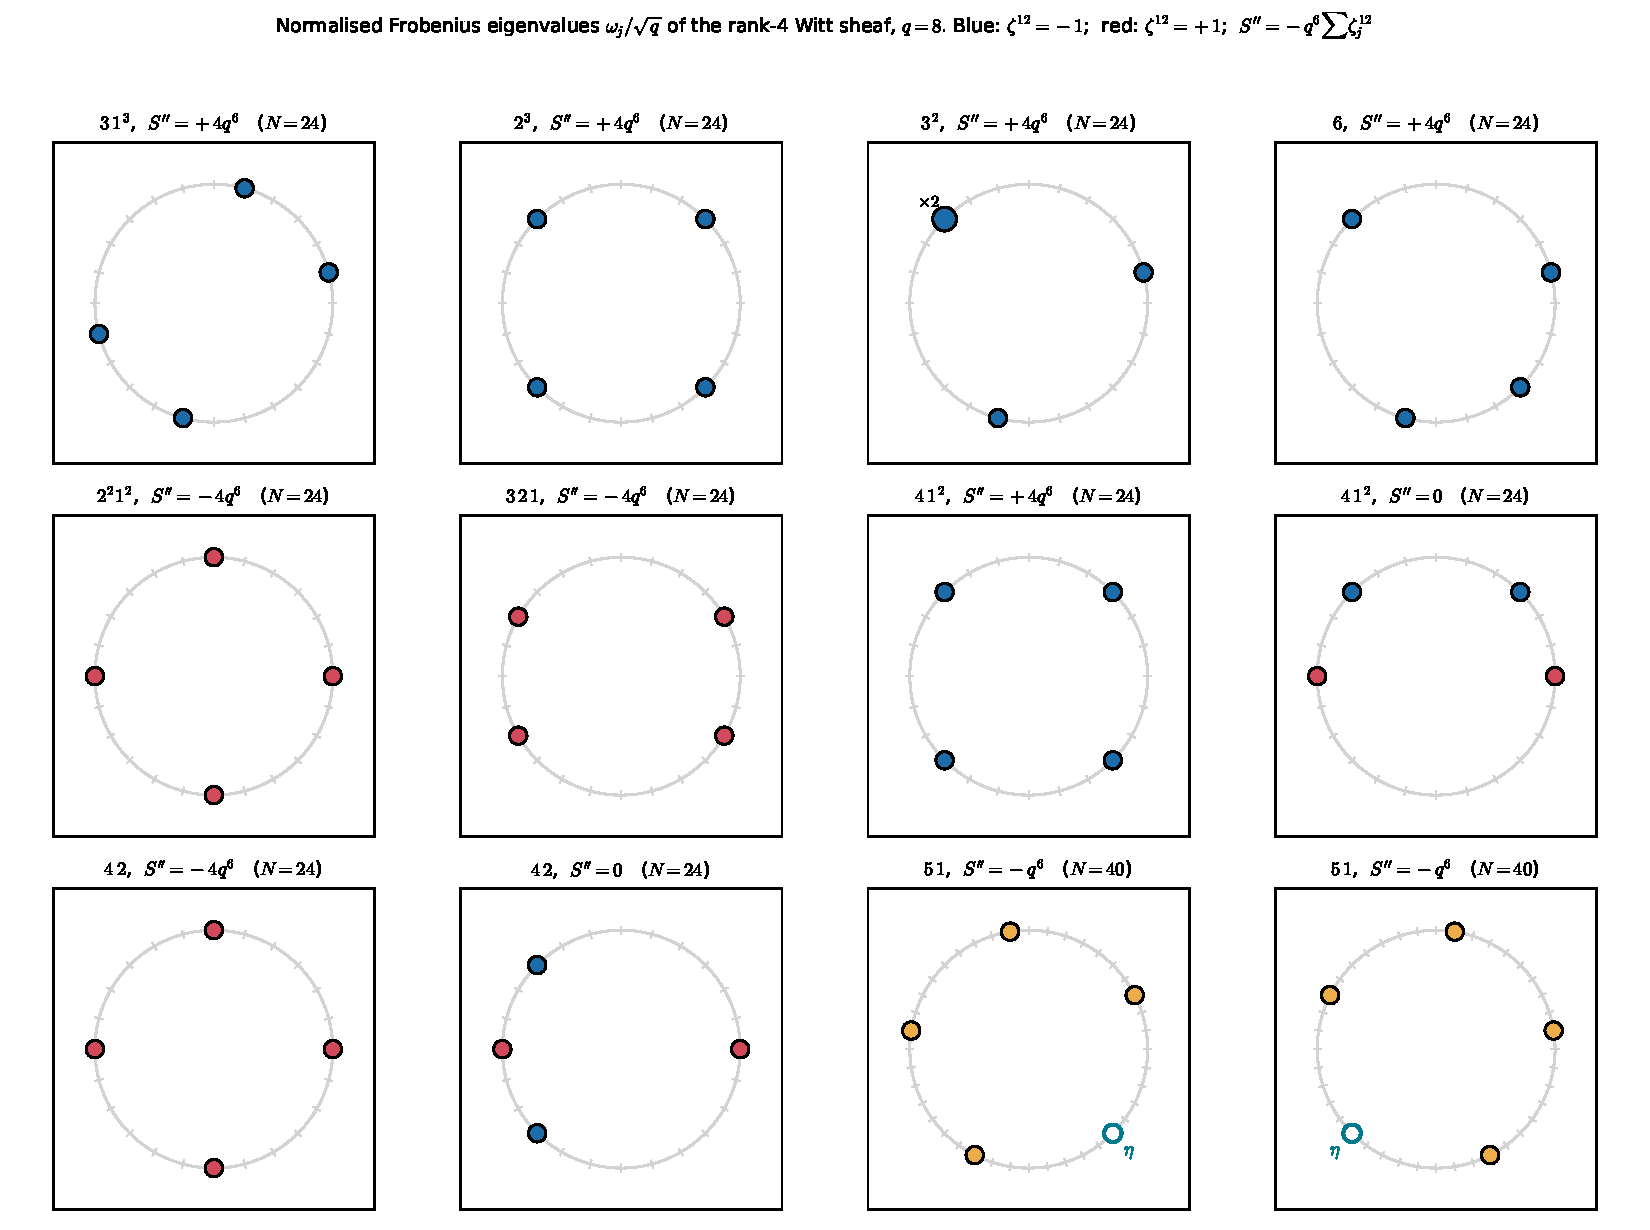
\includegraphics[width=\textwidth]{fig_eigen_circles.pdf}
\caption{Normalised Frobenius eigenvalues of the Witt sheaf for one representative of each (class, value of $\Spp$) at $q=8$ (Table~\ref{tab:eigen}). Blue points have $\zeta^{12}=-1$, red points $\zeta^{12}=+1$; $\Spp=-q^6\sum\zeta_j^{12}$. In the class $5\,1$ the four eigenvalues are the nontrivial $5$th-root translates of the primitive $8$th root $\eta=s_1/\sqrt q$ (open circle), as Theorem~\ref{thm:fivecycle} predicts.}\label{fig:eigen}
\end{figure}

\begin{remark}[reading the tables]
Several of the regularities in Tables~\ref{tab:eigen}--\ref{tab:smallgauss} are theorems proved above, and the others are precise targets. (1) In the class $2^3$, and in the class $2^21^2$ when $\Spp=+4q^6$, $s_2$ is $0$ or $\pm4qi$, never $\pm4q$: indeed if $s_2=\pm4q$ then all $\zeta_j^2=\mp1$, $\zeta_j^4=1$ and $\Spp=-4q^6$. (2) In the classes of order $4$ with $\Spp=0$ one has $s_1\ne0$ (radical $\langle\tau_0\rangle$, $f_1=1$), while for $\Spp\ne0$, $s_1=s_2=s_3=0$: the hyperplane of Theorem~\ref{thm:N0div4} is the complement of the hyperplane on which $\qq^{(1)}_\lambda$ vanishes on $\tau_0$. We have not proved this complementarity. (3) In the class $3\,1^3$, $s_4=-2q^2$ always ($f_4=2$) and $s_3$ vanishes for three quarters of the $\lambda_1$; when it does not, $b_3$ is odd, as Theorem~\ref{thm:N0div6}(ii) requires. (4) In the classes $3^2$ and $6$ the first Gauss sum $s_1$ has trivial radical and is therefore $\sqrt q$ times a primitive $8$th root of unity, exactly as in the class $5\,1$; the difference is that $f_3>0$ there, so the rigidity argument of Theorem~\ref{thm:fivecycle} does not apply.
\end{remark}

\section{Status and open problems}\label{sec:open}

\begin{table}[H]
\centering
\caption{What is proved, what is verified, what is conjectural.}\label{tab:status}
\footnotesize
\begin{tabular}{@{}p{0.55\textwidth}p{0.22\textwidth}p{0.17\textwidth}@{}}
\toprule
statement & status & where\\
\midrule
$\Kk_\lambda=\{0\}\cup\{r_i+r_j\}$ for the roots of $B_\lambda=uA_\lambda+1$; $T'_\lambda(r_i)=1$; deformation $uA_\lambda+\delta$ & proved, all $k$ & Thms~\ref{thm:hexad}, \ref{thm:deform}\\
Frobenius class $=$ factorisation type of $B_\lambda$; orbit structures, $N_0$, $f_m$ & proved, all $k$ & Thm~\ref{thm:classes}\\
Number of $\sigma$-stable symplectic forms of each type $=28|t|/|C|$ & proved; data $q=8,32$ & Prop.~\ref{prop:symplectic}\\
Moments $(q-1)^2$, $(q-2)^2$, $q(q-2)$; pair lemma $\Tr(r+s)=0$ & proved, all $k$ & Thm~\ref{thm:moments}\\
Class counts, $k$ odd (Table~\ref{tab:counts}) & verified $q\le512$; $\lambda_3=0$ proved & Conj.~\ref{conj:counts}\\
Class counts, $k$ even (Table~\ref{tab:evenk}) & fitted to $q\le256$ & \S\ref{subsec:evenk}\\
$\Spp(\lambda)\in\Z$, $\in\{0,\pm4q^6\}$ or $\pm q^6$; $\Spp(\lambda_1)=\Spp(\lambda_1+1)$ & proved, all $k$ & Prop.~\ref{prop:real}\\
$|\omega_j|=\sqrt q$, $\omega_j^{4N_0}$ all equal, $\zeta_j$ roots of unity & proved, all $k$ & Thm~\ref{thm:rootsofunity}\\
Class $5\,1$: $L$-polynomial, $\Spp=(-1)^{k+1}q^6$, $W'=(-1)^{k+1}q^7$ & proved, all $k$ & Thms~\ref{thm:fivecycle}, \ref{thm:evenk}\\
$N_0\mid4$: $\Spp=q^4s_4$; nonvanishing pattern ($q$ or $q/2$ values) & proved, all $k$ & Thm~\ref{thm:N0div4}\\
$N_0\in\{3,6\}$: $\Spp=\pm4q^6$ for all $\lambda_1$; $+$ if $s_3\ne0$ ($k$ odd) & proved & Thm~\ref{thm:N0div6}\\
Sign pattern in $\lambda_1$ is an $\F_2$-quadratic form on $T'_\lambda(V_\lambda)$ & proved & Prop.~\ref{prop:phase}\\
Signs of $s_4$ ($N_0\mid4$), $s_6$ ($N_0\in\{3,6\}$); $W'$ by class & $W'$ verified $q\le128$; $s_m$, $\Spp(\lambda_1)$ at $q=8,32$ & Conj.~\ref{conj:signs}\\
$X=q^6+q^5$ ($k$ odd) & $\Leftarrow$ Conj.~\ref{conj:counts} $+$ Conj.~\ref{conj:signs} & Cor.~\ref{cor:X}\\
\bottomrule
\end{tabular}
\end{table}

\begin{enumerate}[label=\textbf{Open Problem \arabic*.},wide,labelindent=0pt,itemsep=0.8ex]
\item\label{op:counts} Prove Table~\ref{tab:counts}: the factorisation statistics of the family $u^6+au^2+bu+b^2$ over $\F_q$, $q=2^k$, $k$ odd. The four relations of Corollary~\ref{cor:relations} are proved; the remaining moments are point counts of explicit curves which the table predicts to be polynomial.
\item\label{op:brown} Evaluate the Brown invariants of \S\ref{subsec:remains}: the sign of $s_4(\lambda)$ for $N_0\mid4$ and the value of $s_6(\lambda)/4q^3$ for $N_0\in\{3,6\}$ (Conjecture~\ref{conj:signs}). The forms are explicit: $\qq^{(4)}_\lambda$ on $\F_{q^4}$ with radical $\Kk_\lambda$, and $\qq^{(6)}_\lambda$ on $\F_{q^6}$; by the shift calculus the value for one $\lambda_1$ in each coset of $T'_\lambda(\F_q)$ suffices. Together with Open Problem~\ref{op:counts} this would complete the proof of $X=q^6+q^5$ for odd $k$.
\item Extend to even $k$. The hexad theorem and Theorems~\ref{thm:rootsofunity}, \ref{thm:N0div4}, \ref{thm:N0div6}(i),(iii),(iv) hold verbatim; in Theorem~\ref{thm:fivecycle} the parity enters through Lemma~\ref{lem:oddgauss} and gives $\Spp=+q^6$, in agreement with the sign $(-1)^{k+1}$ of Part~II; the class counts must change since the Gold quintic has different statistics for even $k$.
\item Interpret the hexad. The six roots of $B_\lambda$ are attached to the supersingular curve $y^2+y=\lambda_5x^5+\lambda_3x^3$ (they do not depend on $\lambda_1$), and $\Sp_4(\F_2)\cong S_6$ is the automorphism group of the $2$-torsion of a principally polarised abelian surface with its Weil pairing, the six roots playing the role of the Weierstrass points of a genus-two curve. In characteristic $2$ the Jacobian of a supersingular genus-two curve has no \'etale $2$-torsion, and $(\Kk_\lambda,\omega)$ should be a substitute: the $2$-torsion of a lift, or an \'etale piece of a Dieudonn\'e-type object attached to the rank-four Witt sheaf. A conceptual explanation along these lines would presumably also explain the exact class counts and the Brown invariants.
\item Prove that the phase form $\bar Q$ of Proposition~\ref{prop:phase} is linear, i.e.\ $\Tr_{q/2}\bigl(\tau(c)\,T'_\lambda(c')\bigr)=0$ for all $c,c'\in V_\lambda$; and prove the complementarity observed in the classes of order $4$ (Remark after Table~\ref{tab:smallgauss}): $\Spp(\lambda_1)\ne0$ iff $s_1(\lambda_1)=0$.
\item Explain the dependence of the even-$k$ class counts on $k$ modulo $4$ (Table~\ref{tab:evenk}) and prove them; the odd-$k$ counts do not depend on $k$ modulo $4$ although $q\equiv2,3\pmod5$ alternates.
\item The deformation $uA_\lambda(u)+\delta$ (Theorem~\ref{thm:deform}) connects the quadratic sums $W$ of $A_6$ ($\delta=0$) and the order-$4$ sums $W'$ of $X$ ($\delta=1$). For intermediate $\delta$ the sums have no character-sum meaning; but the family of sextics does, and its monodromy ($S_5\subset S_6$ at the boundary) may explain why the quintic statistics of Part~II (three classes) specialise the sextic statistics (eleven classes) exactly as in the column $\lambda_3=0$ of Table~\ref{tab:counts}.
\end{enumerate}

\section*{Acknowledgements}
The computations were carried out with NumPy and SymPy; the search that found $B_\lambda$ (\S\ref{sec:numerics}) was designed and run in an interactive session with Claude (Anthropic), which also assisted with the drafting of the manuscript.

\appendix

\section{All pairs at \texorpdfstring{$q=8$}{q=8}}\label{app:k3}
Table~\ref{tab:k3} lists, for $q=8$, every $(\lambda_3,\lambda_5)\in\F_8\times\F_8^\times$ with the factorisation type of $B_\lambda$ over $\F_8$ and the exact value of $W'(\lambda_3,\lambda_5)/q^7$ from Part~II. Here $\F_8=\F_2[\alpha]/(\alpha^3+\alpha+1)$. Among the $49$ pairs with $\lambda_3\ne0$ the classes $3\,1^3$, $2^21^2$, $3^2$, $4\,1^2$, $4\,2$, $3\,2\,1$, $5\,1$, $6$ occur $3,3,3,3,6,9,13,9$ times, and among the $7$ pairs with $\lambda_3=0$ the classes $4\,1^2$, $2^3$, $6$ occur $3,1,3$ times, in agreement with Table~\ref{tab:counts} at $q=8$ (where $(q-2)(q-8)=0$ kills the classes $1^6$, $2\,1^4$ and the mixed part of $2^3$). The values of $W'$ are constant on the classes, as Theorem~\ref{thm:witt} and Conjecture~\ref{conj:signs} assert; the total $\sum W'=q^9+q^8-W'(0,0)=q^9+q^8-q^7$ over the $56$ pairs gives $X=q^6+q^5=294912$.

\begin{table}[H]
\centering
\caption{$q=8$: all pairs $(\lambda_3,\lambda_5)$, the class of $B_\lambda$ and $W'/q^7$ (generated by \texttt{appendix\_table\_k3.py}).}\label{tab:k3}
\footnotesize
\begin{tabular}{@{}cccc@{\qquad\qquad}cccc@{}}
\toprule
$\lambda_3$ & $\lambda_5$ & class & $W'/q^7$ & $\lambda_3$ & $\lambda_5$ & class & $W'/q^7$\\
\midrule
$\alpha$ & $\alpha^2+\alpha+1$ & $2^21^2$ & $0$ & $\alpha$ & $\alpha+1$ & $4\,2$ & $-2$\\
$\alpha^2$ & $\alpha+1$ & $2^21^2$ & $0$ & $\alpha^2$ & $\alpha^2+1$ & $4\,2$ & $-2$\\
$\alpha^2+\alpha$ & $\alpha^2+1$ & $2^21^2$ & $0$ & $\alpha^2+\alpha$ & $\alpha^2+\alpha+1$ & $4\,2$ & $-2$\\
$0$ & $1$ & $2^3$ & $4$ & $1$ & $1$ & $5\,1$ & $-1$\\
$\alpha+1$ & $\alpha^2+\alpha$ & $3\,1^3$ & $4$ & $\alpha$ & $\alpha$ & $5\,1$ & $-1$\\
$\alpha^2+1$ & $\alpha$ & $3\,1^3$ & $4$ & $\alpha+1$ & $1$ & $5\,1$ & $-1$\\
$\alpha^2+\alpha+1$ & $\alpha^2$ & $3\,1^3$ & $4$ & $\alpha+1$ & $\alpha+1$ & $5\,1$ & $-1$\\
$\alpha$ & $1$ & $3\,2\,1$ & $0$ & $\alpha+1$ & $\alpha^2+\alpha+1$ & $5\,1$ & $-1$\\
$\alpha$ & $\alpha^2+1$ & $3\,2\,1$ & $0$ & $\alpha^2$ & $\alpha^2$ & $5\,1$ & $-1$\\
$\alpha+1$ & $\alpha^2$ & $3\,2\,1$ & $0$ & $\alpha^2+1$ & $1$ & $5\,1$ & $-1$\\
$\alpha^2$ & $1$ & $3\,2\,1$ & $0$ & $\alpha^2+1$ & $\alpha+1$ & $5\,1$ & $-1$\\
$\alpha^2$ & $\alpha^2+\alpha+1$ & $3\,2\,1$ & $0$ & $\alpha^2+1$ & $\alpha^2+1$ & $5\,1$ & $-1$\\
$\alpha^2+1$ & $\alpha^2+\alpha$ & $3\,2\,1$ & $0$ & $\alpha^2+\alpha$ & $\alpha^2+\alpha$ & $5\,1$ & $-1$\\
$\alpha^2+\alpha$ & $1$ & $3\,2\,1$ & $0$ & $\alpha^2+\alpha+1$ & $1$ & $5\,1$ & $-1$\\
$\alpha^2+\alpha$ & $\alpha+1$ & $3\,2\,1$ & $0$ & $\alpha^2+\alpha+1$ & $\alpha^2+1$ & $5\,1$ & $-1$\\
$\alpha^2+\alpha+1$ & $\alpha$ & $3\,2\,1$ & $0$ & $\alpha^2+\alpha+1$ & $\alpha^2+\alpha+1$ & $5\,1$ & $-1$\\
$\alpha$ & $\alpha^2$ & $3^2$ & $4$ & $0$ & $\alpha$ & $6$ & $4$\\
$\alpha^2$ & $\alpha^2+\alpha$ & $3^2$ & $4$ & $0$ & $\alpha^2$ & $6$ & $4$\\
$\alpha^2+\alpha$ & $\alpha$ & $3^2$ & $4$ & $0$ & $\alpha^2+\alpha$ & $6$ & $4$\\
$0$ & $\alpha+1$ & $4\,1^2$ & $2$ & $1$ & $\alpha+1$ & $6$ & $4$\\
$0$ & $\alpha^2+1$ & $4\,1^2$ & $2$ & $1$ & $\alpha^2+1$ & $6$ & $4$\\
$0$ & $\alpha^2+\alpha+1$ & $4\,1^2$ & $2$ & $1$ & $\alpha^2+\alpha+1$ & $6$ & $4$\\
$\alpha+1$ & $\alpha$ & $4\,1^2$ & $2$ & $\alpha$ & $\alpha^2+\alpha$ & $6$ & $4$\\
$\alpha^2+1$ & $\alpha^2$ & $4\,1^2$ & $2$ & $\alpha+1$ & $\alpha^2+1$ & $6$ & $4$\\
$\alpha^2+\alpha+1$ & $\alpha^2+\alpha$ & $4\,1^2$ & $2$ & $\alpha^2$ & $\alpha$ & $6$ & $4$\\
$1$ & $\alpha$ & $4\,2$ & $-2$ & $\alpha^2+1$ & $\alpha^2+\alpha+1$ & $6$ & $4$\\
$1$ & $\alpha^2$ & $4\,2$ & $-2$ & $\alpha^2+\alpha$ & $\alpha^2$ & $6$ & $4$\\
$1$ & $\alpha^2+\alpha$ & $4\,2$ & $-2$ & $\alpha^2+\alpha+1$ & $\alpha+1$ & $6$ & $4$\\
\bottomrule
\end{tabular}

\end{table}

\section{Algorithms and run times}\label{app:algo}
\textbf{Fields.} $\F_{q^{12}}$ is represented as $\F_q[z]/(m(z))$ with $m$ irreducible of degree $12$ over $\F_q$ (fqlib tables of Part~II), and every $\F_2$-linear map ($x\mapsto x^2$, $x\mapsto x^{1/2}$, multiplication by a constant, $\Tr_{q^{12}/q}$, $T'_\lambda$) is stored as a $12k\times12k$ matrix over $\F_2$; $\Kk_\lambda$ is the nullspace of the matrix of $L'_\lambda=(T'_\lambda)^4$, computed by Gaussian elimination over $\F_2$.

\textbf{Hexad search.} The $168$ frames of $\Kk_\lambda$ are the $4$-subsets of $\Kk_\lambda\setminus0$ of rank $4$ completed by their sum (there are $\binom{15}4=1365$ subsets, $840$ of rank $4$, and each frame arises from its $5$ four-subsets); a frame $F$ gives the hexad $H=\{0\}\cup F$, whose translation class is tested for $\sigma$-stability by checking whether $\sigma(H)+h\in\{H+v:v\in\Kk_\lambda\}$ for some $h$. For a stable class the polynomial $\prod_{h\in H}(u+h)$ is computed, the translate killing the $u^4$-coefficient is taken, and the coefficients are tested for membership in $\F_q$. Cost per pair: $O(168\cdot16)$ polynomial evaluations in $\F_{q^{12}}$; run times a few seconds ($q=8$), $5$\,min ($q=32$), several hours ($q=128$, $16256$ pairs).

\textbf{Class counts.} \texttt{sextic\_types.py} computes $\gcd(B_\lambda,u^{q^m}-u)$, $m=1,\dots,6$, by repeated squaring modulo $B_\lambda$ over $\F_q$; run times under a second for $q=8,32$, $11$\,s for $q=128$ and $5$\,min for $q=512$.

\textbf{Witt sums.} For $m\le4$ the field $\F_{2^{mk}}$ is given by log/exp tables; the Witt trace $\mathsf T_{mk}(x)$ of all $2^{mk}-1$ nonzero $x$ at once is accumulated by the vectorised recursion $(s_0,s_1)\leftarrow(s_0+c,\ s_1+s_0c)$ over the $mk$ conjugates $c=x,x^2,\dots$ (this is \eqref{eq:T} evaluated by Horner-type accumulation of the Witt sum), and $2\Tr_{q^m/2}f_\lambda(x)$ is added; the Gauss sum is then a histogram of the four values. Cost $O(mk\,2^{mk})$ per $(\lambda,m)$; for $q=8$ all $448$ values of $\lambda$ take $2.5$\,min and for $q=16$ all $3840$ values about $50$\,min; at $q=32$ the sums with $m=4$ run over $\F_{2^{20}}$ and the sample of four pairs per class ($1408$ values of $\lambda$) took about two hours. Newton's identities over $\Q(i)$ give the $e_j$ of the $\omega_j$ from $s_1,\dots,s_4$; the roots are computed numerically and recognised as $\sqrt q$ times roots of unity (exponents on a common denominator $120$), and $\Spp=-\sum\omega_j^{12}$ is evaluated exactly from the power sums.

\textbf{Reference values.} The exact $W'(\lambda_3,\lambda_5)$ are those of Part~II, obtained from the $\F_2$-quadratic form $Q'$ on $\F_{q^{12}}$ by the radical algorithm (\texttt{legendre\_d6\_qf.py}); the agreement $\sum_{\lambda_1}\Spp(\lambda)=W'$ in every case is therefore a check of two independent computations (Witt sums over $\F_{q^m}$, $m\le4$, against an $\F_2$-form over $\F_{q^{12}}$) as well as of the $L$-polynomial principle.

\clearpage
\begin{thebibliography}{99}
\bibitem{Bluher} A.~W.~Bluher, \emph{On $x^{q+1}+ax+b$}, Finite Fields Appl.\ \textbf{10} (2004), 285--305.
\bibitem{Brown} E.~H.~Brown, \emph{Generalizations of the Kervaire invariant}, Ann.\ of Math.\ (2) \textbf{95} (1972), 368--383.
\bibitem{Brylinski} J.-L.~Brylinski, \emph{Th\'eorie du corps de classes de Kato et rev\^etements ab\'eliens de surfaces}, Ann.\ Inst.\ Fourier \textbf{33} (1983), 23--38.
\bibitem{Chen} R.~Chen, \emph{Primes in Legendre intervals over $\F_q[t]$: an exact explicit-formula algorithm, verification for $d\le10$, and an anomaly in characteristic~2}, preprint (2026), DOI 10.5281/zenodo.23225896.
\bibitem{ChenII} R.~Chen, \emph{Prime polynomials in Legendre intervals over $\F_{2^k}[t]$, II: exact variances via quadratic towers and supersingular Artin--Schreier curves}, preprint, version 2 (2026), DOI 10.5281/zenodo.23252762.
\bibitem{Conway} J.~H.~Conway, R.~T.~Curtis, S.~P.~Norton, R.~A.~Parker and R.~A.~Wilson, \emph{Atlas of Finite Groups}, Oxford University Press, 1985.
\bibitem{Deligne} P.~Deligne, \emph{La conjecture de Weil. II}, Publ.\ Math.\ IH\'ES \textbf{52} (1980), 137--252.
\bibitem{GV} G.~van der Geer and M.~van der Vlugt, \emph{Reed--Muller codes and supersingular curves. I}, Compositio Math.\ \textbf{84} (1992), 333--367.
\bibitem{HK} T.~Helleseth and A.~Kholosha, \emph{On the equation $x^{2^l+1}+x+a=0$ over $GF(2^k)$}, Finite Fields Appl.\ \textbf{14} (2008), 159--176.
\bibitem{Katz} N.~M.~Katz, \emph{Witt vectors and a question of Keating and Rudnick}, Int.\ Math.\ Res.\ Not.\ IMRN (2013), 3613--3638.
\end{thebibliography}

\end{document}
